\chapter{RFD and MRAI correlation}
\label{cha:bgp_rfd}

%\begin{itemize}
%    \item Expose more deeply what is RFD
%    \item Expose previous studies about RFD
%    \item Today RFD? Outdated
%\end{itemize}

\ac{RFD} is another parameter of \ac{BGP} used to avoid messages storms.
It is used to avoid flapping routes to continuously make the network unstable.
When a network flaps a certain value is increased and when it overpass a threshold
then the route is suppressed and not advertised anymore until it goes back
below the threshold (or after a certain time).

\ac{RFD}, other than \ac{MRAI}, is one of the most studied parameters of \ac{BGP}
because of its influence in the convergence time \cite{mao2002route,pelsser2011route}.
\ac{RFD} received different updates from its first implementation, but recent 
studies showed that most of the providers still use outdated parameters \cite{gray2020bgp}.

The use of deprecated values can lead to a heavy restrictive suppression
of small routes delaying the correct spreading of information.
Some cases of suppression are caused by faulty interfaces that heavily flaps hundreds of times, 
while other times is just an update of the node configuration that
cause the route to flaps a couple of times and still be suppressed.

In the following chapters, I am going to show how legacy \ac{RFD} can affect 
small flaps and how would the new version of \ac{RFD} react to them.
Finally, I would look forward to understand the correlation between \ac{RFD}
and \ac{MRAI}.
When a suppressed route is shared again it could provoke messages storms that
triggers different \ac{MRAI} session, or the opposite case, a low \ac{MRAI} that
cause the growth of the figure of merit that suppresses a route.

\section{RFD on toy topologies}
\label{sec:bgp_rfd_toy}

I firstly studied \ac{RFD} on toy topologies, to see the effects of it in small 
networks, like I did in \Cref{sec:bgp_mrai_clique}.
As a graph, I used a clique of dimension \num{10}, the source of the signalling
is connected to the node \num{0} while the node \num{5} act as unique servicer
for the node $x$.
The node \num{5} won't be able to share information to node $x$ because of \ac{RFD}.
Node $x$ would have to wait until the route fell below the reuse threshold of 
node \num{5} to converge.

The parameters used for \ac{RFD} are the default \textit{CISCO} parameters,
showed in table \Cref{tbl:cisco_rfd}

\begin{table}[h]
	\begin{center}
	\begin{tabular}{ || m{5cm}| m{2cm} || } 
	\hline
	Parameter & Value \\ 
	\hline \hline
	withdrawal penalty & 1.0 \\
	\hline
    re-advertisement penalty & 0.0 \\
	\hline
    attribute change penalty & 1.0 \\
	\hline
    suppress threshold & 2.0 \\
	\hline
    half-life (min) & 15 (900s) \\
	\hline
    Reuse Threshold & 0.75 \\
	\hline
    Max Suppress Time (min.) & 60 (3600s) \\
	\hline
	\end{tabular}
\end{center}

	\caption{Cisco default \ac{RFD} parameters}
	\label{tbl:cisco_rfd}
\end{table}

The parameters of the environment are in \Cref{tbl:clique_rfd_params}

\begin{table}[h]
	\begin{center}
	\begin{tabular}{ || m{4cm}| m{8cm} || } 
	\hline
	Property & Value \\ 
	\hline \hline
	Seeds & $[1, 10]$ \\ 
	\hline
	Signaling & \q{AWAWAWA} \\
	\hline
		Withdraws delay & Constant distribution of \SI{300}{\second} \\ 
	\hline
	Announcement delay & constant distribution of \SI{300}{\second} \\ 
	\hline
		MRAI & $[0, 120]$ \\
	\hline
	Link delay & Uniform distribution between \SI{0.012}{\second} and \SI{3}{\second} \\
	\hline
	\end{tabular}
\end{center}

	\caption{Environment parameters used for the experiments on \ac{RFD}
		with the clique graph}
	\label{tbl:clique_rfd_params}
\end{table}

Messages in the signal are delayed by \SI{300}{\second} for two reasons:
\begin{itemize}
	\item The main goal of these experiments is to study the correlation from
		\ac{RFD} to \ac{MRAI} and we don't want that \ac{MRAI} compress
		parts of the signal.
	\item I'm trying to simulate one of the possible behaviour tat triggers
		\ac{RFD} suppressions, the human faulty reconfiguration of the node.
\end{itemize}

The signals contain \num{3} flaps in it, the first one is hipotetically attributed
to a configuration that doesn't work properly, the second one is caused by a
buggy correction of the configuration and the last one by the introduction of a
correct configuration.

The \ac{MRAI} strategy used in all the experiments is the \textit{fixed} one.

\begin{figure}[h]
     \centering
     \begin{subfigure}[b]{0.45\textwidth}
         \centering
		 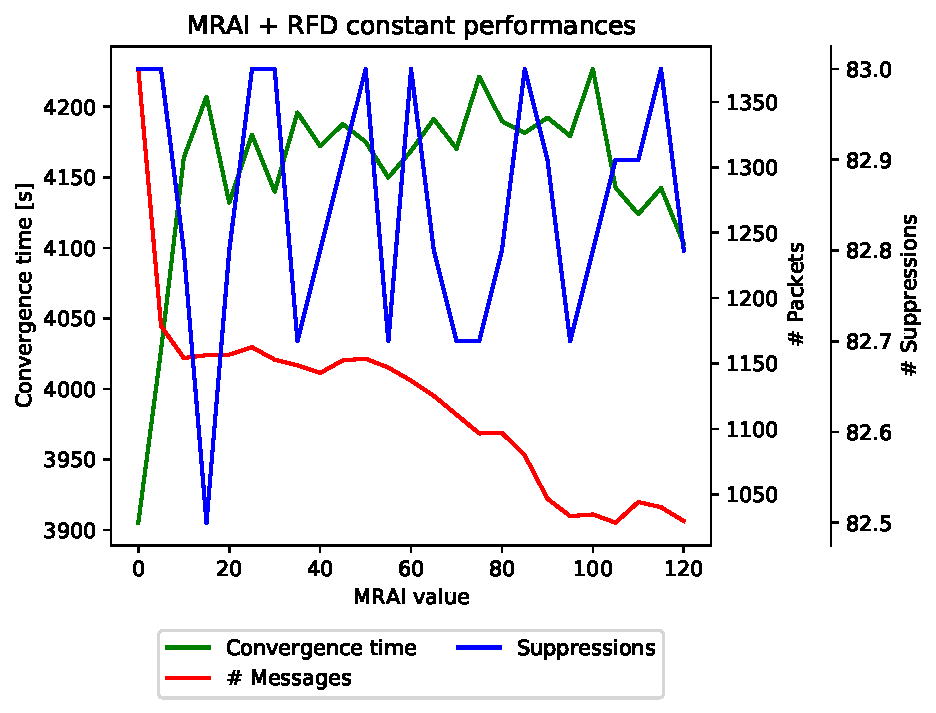
\includegraphics[width=\textwidth]{images/RFD/clique/cisco_clique10_RFD-constant_mrai_rfd_evolution.pdf}
		 \caption{Network performances with the standard cisco \ac{RFD} 
			\fxfatal{redo this plot with a broader range of suppressions $[81-84]$}}
		 \label{fig:clique_evolution_rfd}
     \end{subfigure}
     \hfill
     \begin{subfigure}[b]{0.45\textwidth}
         \centering
         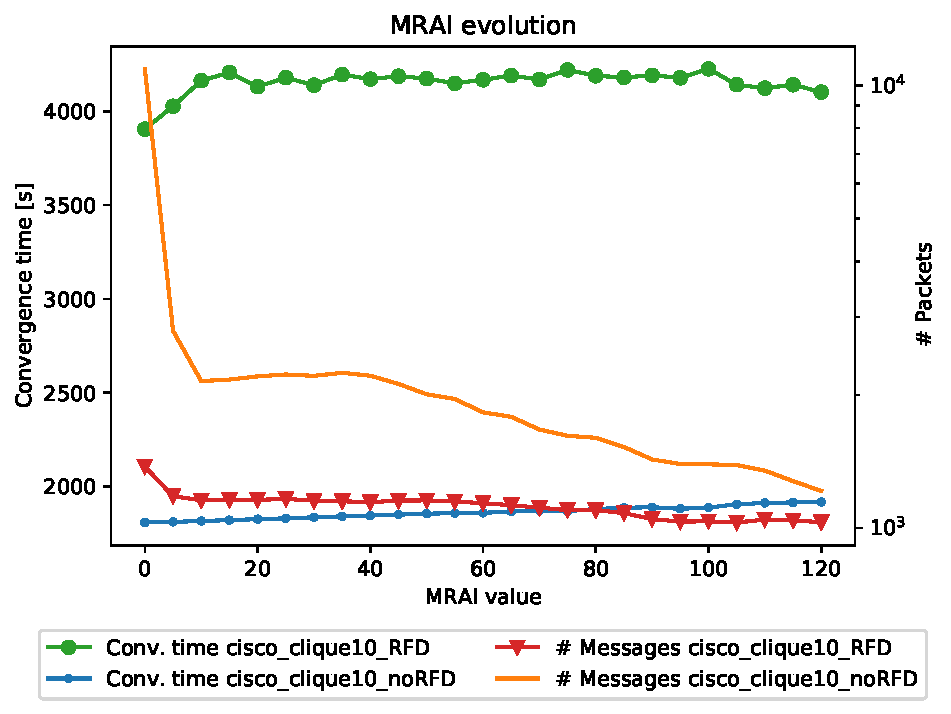
\includegraphics[width=\textwidth]{images/RFD/clique/cisco_clique10_comparison_constant_all.pdf}
		 \caption{Network performances standard \ac{RFD} vs no \ac{RFD}}
         \label{fig:clique_evolution_rfd_vs_noRFd_comparison}
     \end{subfigure}
		\caption{Evolution of the performances changing \ac{MRAI} in the links
			standard \ac{RFD} vs no \ac{RFD},
			graph clique of \num{10} nodes, \ac{MRAI} strategy fixed, signal \q{AWAWAWA}}
        \label{fig:clique_evolution_rfd_vs_noRFD}
\end{figure}

The plot in \Cref{fig:clique_evolution_rfd} contains a third line that represent 
the average total number of suppressions detected on the experiment, for each experiment
has been executed \num{10} different runs.
The blue line that represents the number of suppressions refers to the third y-axis
on the right.

In \cref{fig:clique_evolution_rfd} is possible to see that small changes to \ac{MRAI}
can lead to some small differences in the number of suppressions.
Also, the number of messages decreases rapidly and reaches a constant 
value around \num{1000}, as expected by the passage from an \ac{MRAI} of \SI{0}{\second}
to a few seconds.
The nodes that don't trigger a suppression seems to affect also the
\fxfatal{Explain better the next phrase}
The convergence time stais stable around \SI{4000}{\second} due to the
fact that there are almost the same number of suppressions that takes the same
ammount of time to be solved

In \Cref{fig:clique_evolution_rfd_vs_noRFd_comparison} is possible to see the
gap between the use of \ac{RFD} and without it.
Notice that the packet axis is in log scale.
The difference in the convergence time is due to the fact that with \ac{RFD} some
nodes block the best path that takes a lot of time to become available again.
While \ac{MRAI} grows the set of nodes that suppress routes decreases but the
convergence time is highly affected by a restrict subset of them.
In our case, for example, the suppressions on nodes \num{0} and \num{5} plays
an important role.
The first one for the spreading in the whole network, the second one for the
transmission of information to node $x$.

For this reason, we can look more deeply on what happened to the figure of merit
of node $x$ and five in \Cref{fig:clique_nodex,fig:clique_node5}

\begin{figure}[h]
     \centering
     \begin{subfigure}[b]{0.3\textwidth}
         \centering
         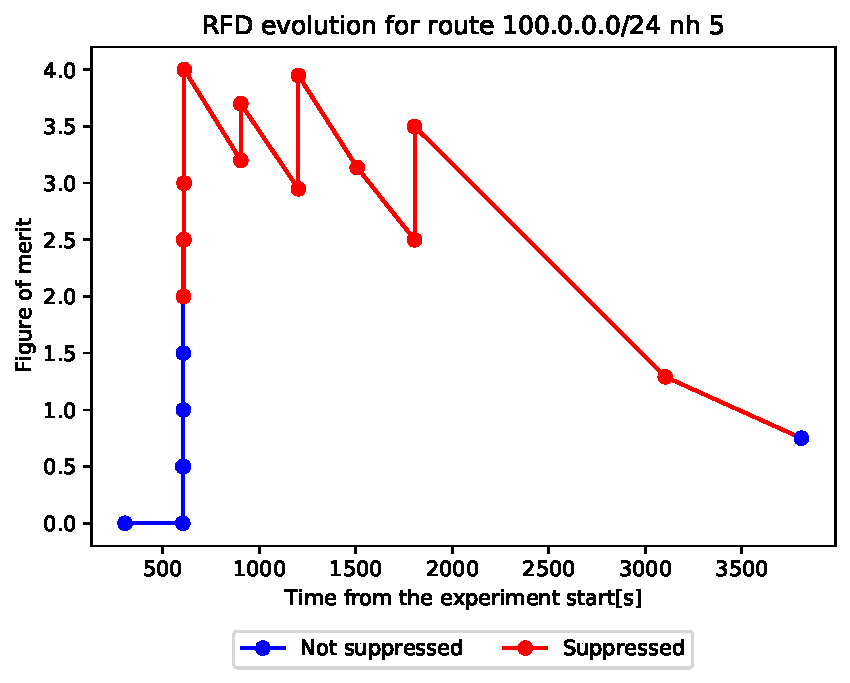
\includegraphics[width=\textwidth]{images/RFD/clique/FigureOfMerit/mrai1_RFD_x_rfd_R1.pdf}
         \caption{MRAI = 0s}
         \label{fig:clique_x_mrai0}
     \end{subfigure}
     \hfill
     \begin{subfigure}[b]{0.3\textwidth}
         \centering
         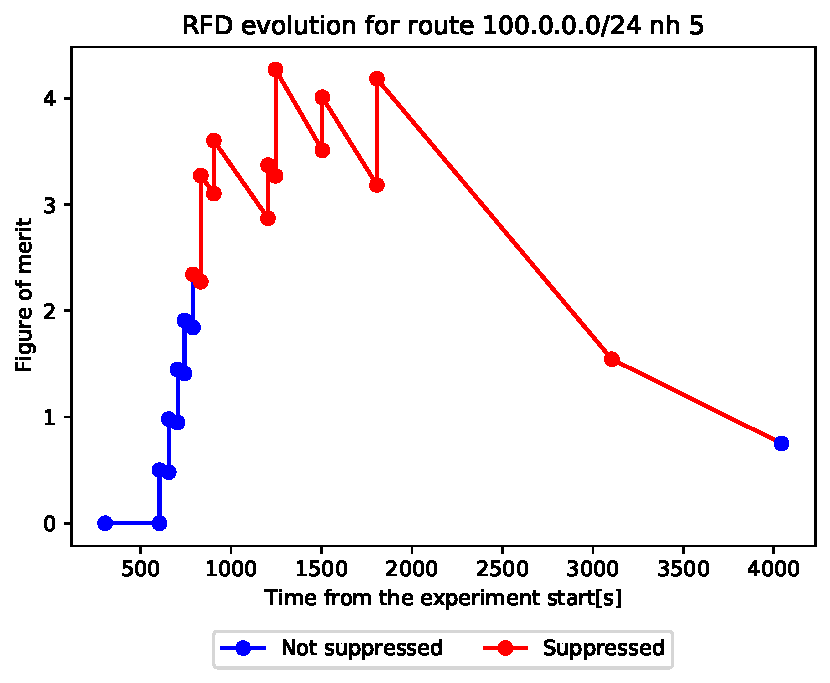
\includegraphics[width=\textwidth]{images/RFD/clique/FigureOfMerit/mrai11_RFD_x_rfd_R1.pdf}
         \caption{MRAI = 50s}
         \label{fig:clique_x_mrai50}
     \end{subfigure}
     \hfill
     \begin{subfigure}[b]{0.3\textwidth}
         \centering
         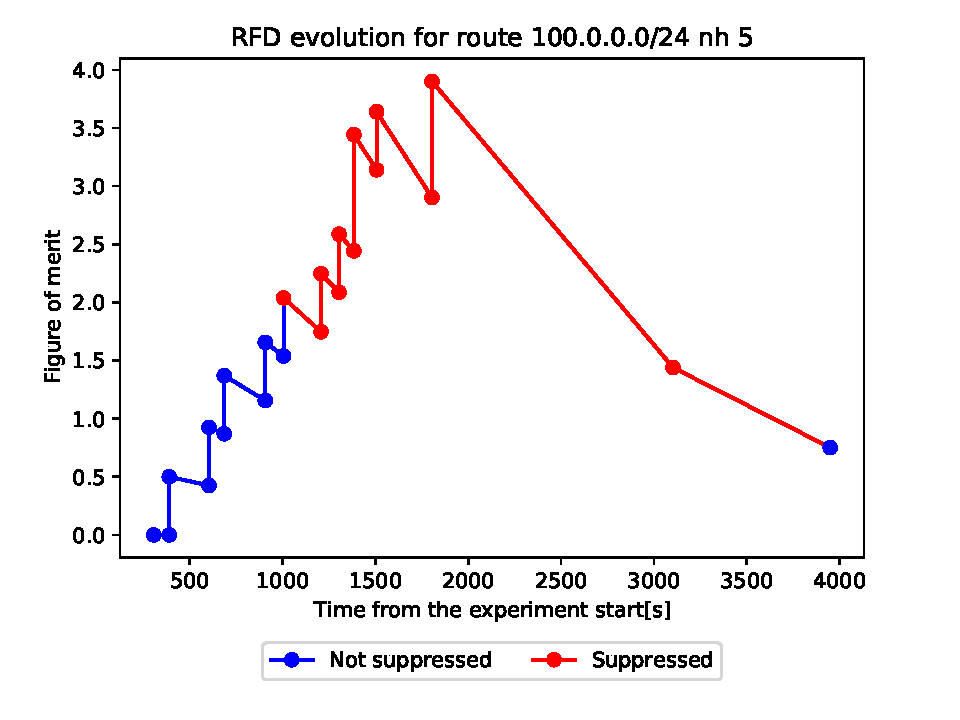
\includegraphics[width=\textwidth]{images/RFD/clique/FigureOfMerit/mrai21_RFD_x_rfd_R1.pdf}
         \caption{MRAI = 100s}
         \label{fig:clique_x_mrai100}
     \end{subfigure}
        \caption{Evolution of the figure of merit in the node X with different MRAIs}
        \label{fig:clique_nodex}
\end{figure}

The node $x$ is a leaf of the network that will absorb everything the node \num{5}
sends to it.
In \Cref{fig:clique_nodex} is possible to see the evolution of the figure of merit
with different \ac{MRAI} values.
In the first case, with an \ac{MRAI} equal to \SI{0}{\second}, we will see a huge
spike caused by a lot of messages and route changes that the node \num{5} sends
to it.
while in the other two cases \Cref{fig:clique_x_mrai50,fig:clique_x_mrai100} 
the \ac{MRAI} seems to not be much effective on the route through node \num{5}.
The messages are more delayed with high \ac{MRAI} but the growth of the figure
of merit has the same trend.
In those cases, we can see that the route has been suppressed around \SI{1000}{\second}
and is going to become useful again around \SI{4000}{\second}.
In this period of time from \SI{1000}{\second} to \SI{4000}{\second}, node $x$ still
receives some updates from node \num{5} that affects its best path, and this
makes the figure of merit evolve.
The evolution of the figure of merit stops around \SI{2000}{\second} that's because
also the node \num{5} has suppressed the route, \Cref{fig:clique_node5}, and
doesn't send any more advertisements.
The point around \SI{3000}{\second} represent the moment when the route becomes
available again for node \num{5} that communicates the change to $x$.

\begin{figure}[h]
     \centering
     \begin{subfigure}[b]{0.3\textwidth}
         \centering
         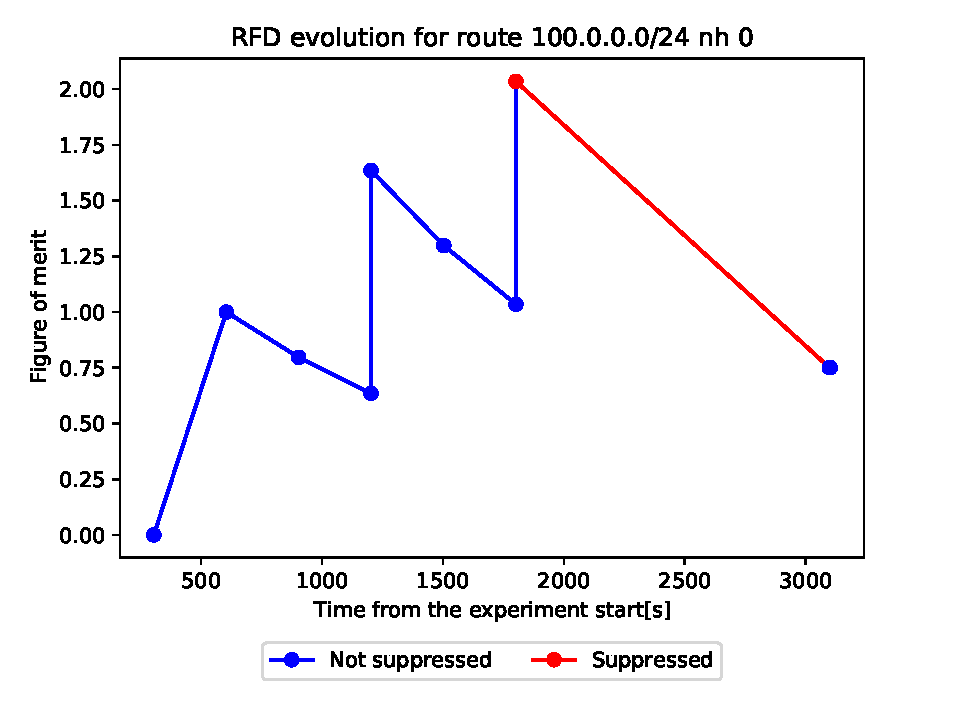
\includegraphics[width=\textwidth]{images/RFD/clique/FigureOfMerit/mrai1_RFD_5_rfd_R1.pdf}
         \caption{MRAI = 0s}
         \label{fig:clique_5_mrai0}
     \end{subfigure}
     \hfill
     \begin{subfigure}[b]{0.3\textwidth}
         \centering
         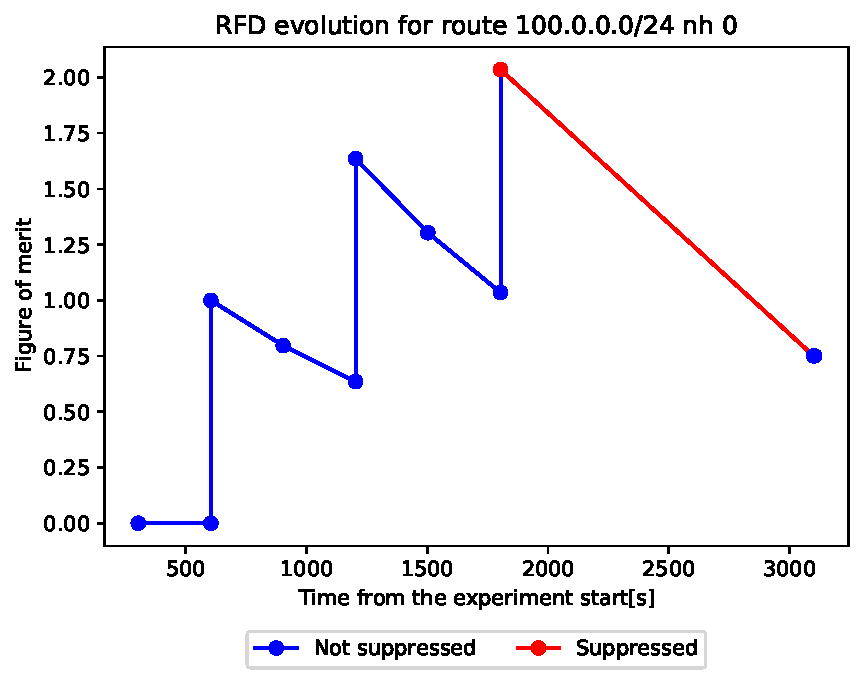
\includegraphics[width=\textwidth]{images/RFD/clique/FigureOfMerit/mrai11_RFD_5_rfd_R1.pdf}
         \caption{MRAI = 50s}
         \label{fig:clique_5_mrai50}
     \end{subfigure}
     \hfill
     \begin{subfigure}[b]{0.3\textwidth}
         \centering
         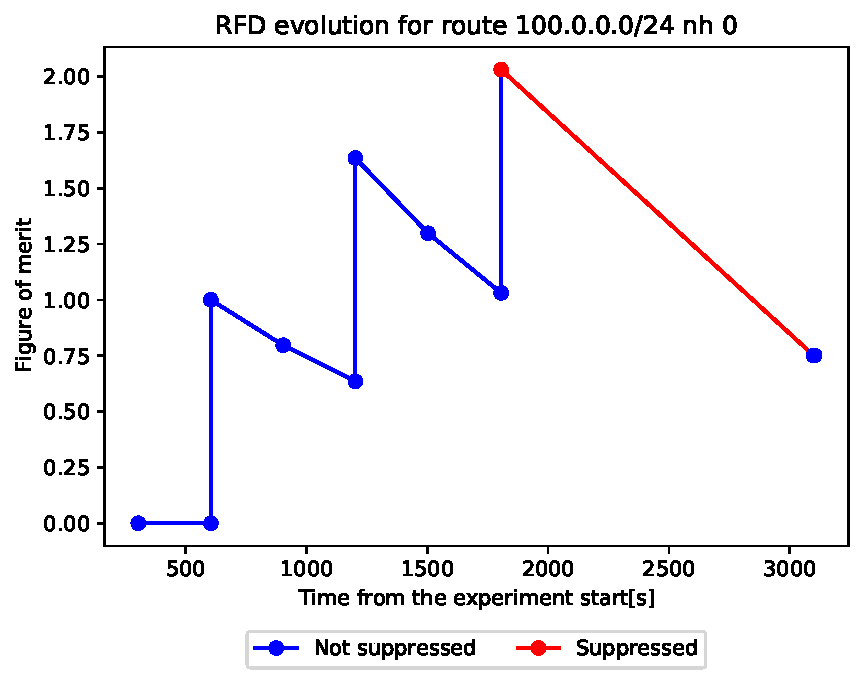
\includegraphics[width=\textwidth]{images/RFD/clique/FigureOfMerit/mrai21_RFD_5_rfd_R1.pdf}
         \caption{MRAI = 100s}
         \label{fig:clique_5_mrai100}
     \end{subfigure}
        \caption{Evolution of the figure of merit in the node X with different MRAIs}
        \label{fig:clique_node5}
\end{figure}

The evolution of the figure of merit of the best path of node \num{5} is different
from the one of node $x$.
In fact, it is not influenced by \ac{MRAI} as we can see in \Cref{fig:clique_node5}.
That because the node \num{5} is directly connected to the node \num{0} that every
\SI{300}{\second} forward the message of $d$. \SI{300}{\second} are a too large
delay to be affected by the compression effect of \ac{MRAI}.
Around \SI{2000}{\second} node \num{5} suppress the route (as any other node in the
clique) and stops to forward it to node $x$ until \SI{3000}{\second} when it becomes
available again.

Node $x$ took almost \SI{4000}{\second} to converge because of the big fluctuations
of node \num{5} that suffers of the \textit{Path Exploration} problem, path
changes are considered bad behaviour in \ac{RFD}.

In conclusion, we can say that \ac{RFD} can be affected by \ac{MRAI} and
that \ac{RFD} can prevent a lot of messages at the cost of very high convergence
times.

%\begin{itemize}
%    \item What is the impact of RFD?
%    \item In which occasion is present RFD?
%    \item Clique
%    \item Variations thanks to MRAI
%\end{itemize}

\section{RFC 2439 VS RFC 7196}
\label{sec:bgp_rfd_comparison}

The difference in the two \ac{RFC} that defines \ac{RFD} \cite{rfc2439,rfc7196}
is in the parameters used.
Infact the last \ac{RFC} introduce two new set of parameters where the figure
of merit threshold is increased up to at least \num{6.0}.
The two categories are:
\begin{itemize}
	\item \textit{\textbf{Aggressive}}, Suppression threshold no less than \num{6.0};
	\item \textit{\textbf{Conservative}}, Suppression threshold no less than \num{12.0};
\end{itemize}

Respectively \num{3} and \num{6} times the actual standard.

I have then repeated the same experiments of \Cref{sec:bgp_rfd_toy} with the same
clique graph, but with the two new \ac{RFD} strategies, the results are 
showed in \Cref{fig:clique_rfd7196}.

\begin{figure}[h]
     \centering
     \begin{subfigure}[b]{0.48\textwidth}
         \centering
         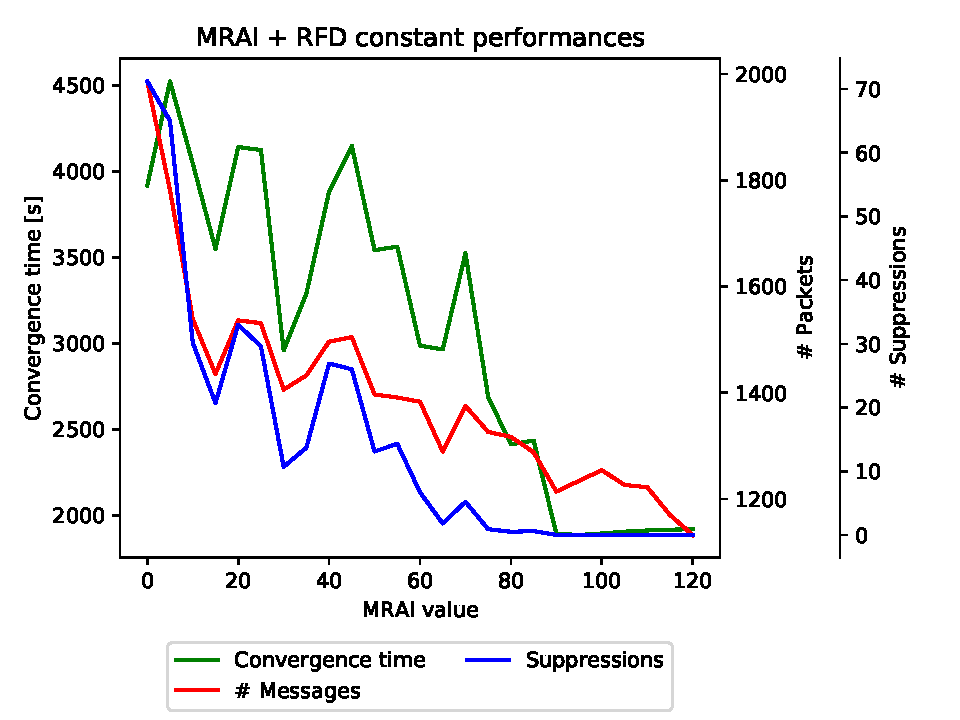
\includegraphics[width=\textwidth]{images/RFD/clique/cisco_clique10_RFD_7196_aggressive-constant_mrai_rfd_evolution.pdf}
         \caption{RFD 7196 Aggressive on the clique topology}
         \label{fig:rfd7196aggressive}
     \end{subfigure}
     \hfill
     \begin{subfigure}[b]{0.48\textwidth}
         \centering
         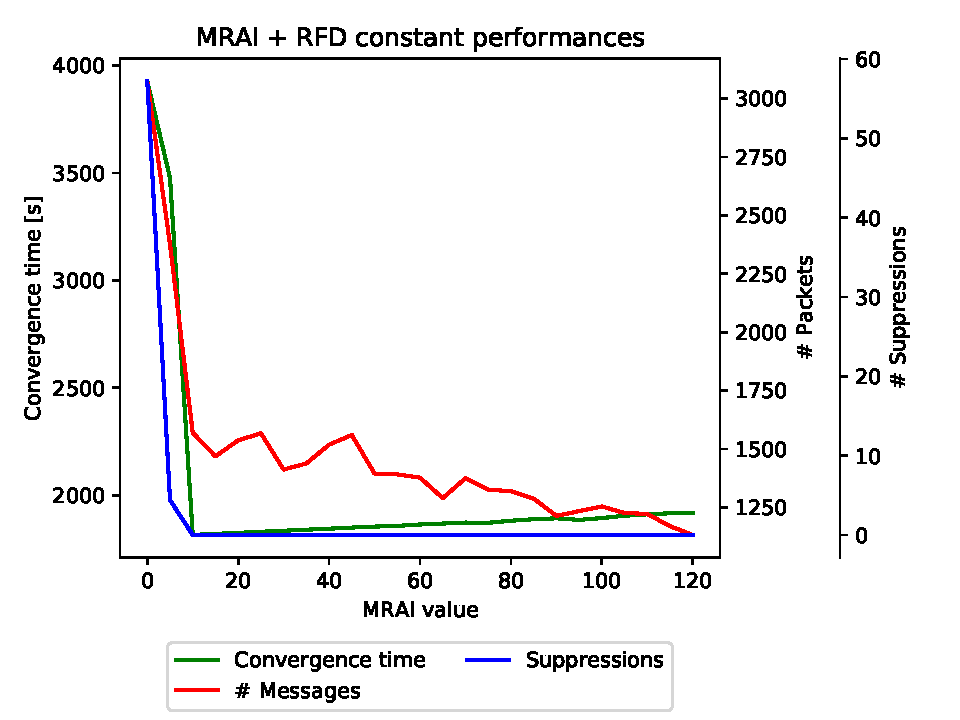
\includegraphics[width=\textwidth]{images/RFD/clique/cisco_clique10_RFD_7196_conservative-constant_mrai_rfd_evolution.pdf}
         \caption{RFD 7196 Conservative on the clique topology}
         \label{fig:rfd7196conservative}
     \end{subfigure}
		\caption{MRAI influence with different RFD strategies from \cite{rfc7196}}
        \label{fig:clique_rfd7196}
\end{figure}

We can see two completely different evolutions of the performances in \Cref{fig:clique_rfd7196}.
On the left plot, we can see the evolution with the \textit{Aggressive} strategy.
and \ac{MRAI} is more effective to this strategy in respect of the standard one.
The number of suppressions fell down to almost \num{0} with an \ac{MRAI} near 
\SI{90}{\second}.
The message trend is similar to the one of the case without \ac{RFD} but with an
important difference in the case of  \ac{MRAI} equal \SI{0}{\second}, the number
of average messages is around \num{2600} in respect of the \num{10000} without
\ac{RFD}.
While with a high \ac{MRAI} the message trends are similar and equal when the number of
suppressions reaches \num{0}.

The convergence time, on the other hand, has a differen trend in respect of 
the one that we saw in \Cref{fig:clique_evolution_rfd}.
Here we see a descending trend caused by the fact that \ac{MRAI} is able to avoid
some messages and, as a consequence, avoid the growing of the figure of merit in 
some nodes permitting to the convergence time to decrease.
Once the number of suppressions reaches \num{0} obviously the network performances
are equal as in the \textit{NoRFD} case.

In \Cref{fig:rfd7196conservative} we can see the evolution of the network with the 
\textit{Conservative} strategy, the threshold of this strategy is the double of
the \textit{Aggressive} strategy.
The effects of this difference are huge, is sufficient an \ac{MRAI} of \SI{10}{\second}
to avoid at all suppressions, causing the trend, in terms of messages and
convergence time to be equal to the no \ac{RFD} case.
Also with an \ac{MRAI} of \SI{0}{\second} is possible to see a difference in 
terms of messages and convergence time in respect of the other two strategies.
This is the strategy that more likely resembles the \textit{NoRFD} one,
having a convergence time incredibly more low, at the cost of few hundreds messages.

We can now take a look more closely to what happens to the figure of merit 
for the only route that node $x$ receives.
Results are exposed in \Cref{fig:clique_nodex_rfd7196Aggressive}

\begin{figure}[h]
     \centering
     \begin{subfigure}[b]{0.3\textwidth}
         \centering
         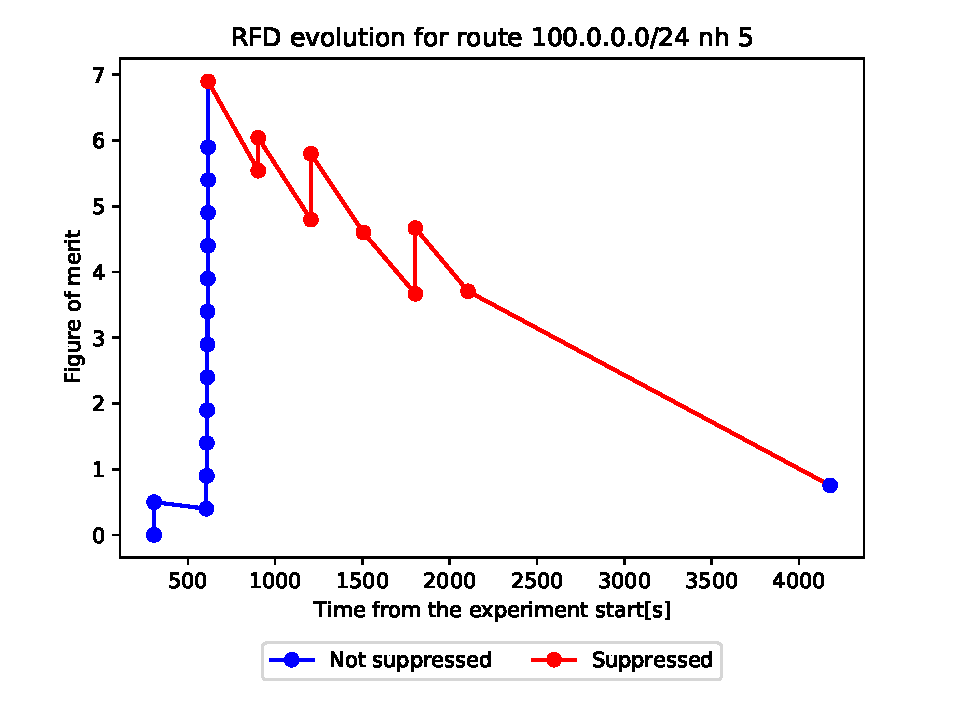
\includegraphics[width=\textwidth]{images/RFD/clique/FigureOfMerit/mrai1_RFD_7196_aggressive_x_rfd_R1.pdf}
         \caption{MRAI = 0s, RFD 7196 Aggressive, clique topology}
         \label{fig:clique_x_mrai0_rfd7196Aggressive}
     \end{subfigure}
     \hfill
     \begin{subfigure}[b]{0.3\textwidth}
         \centering
         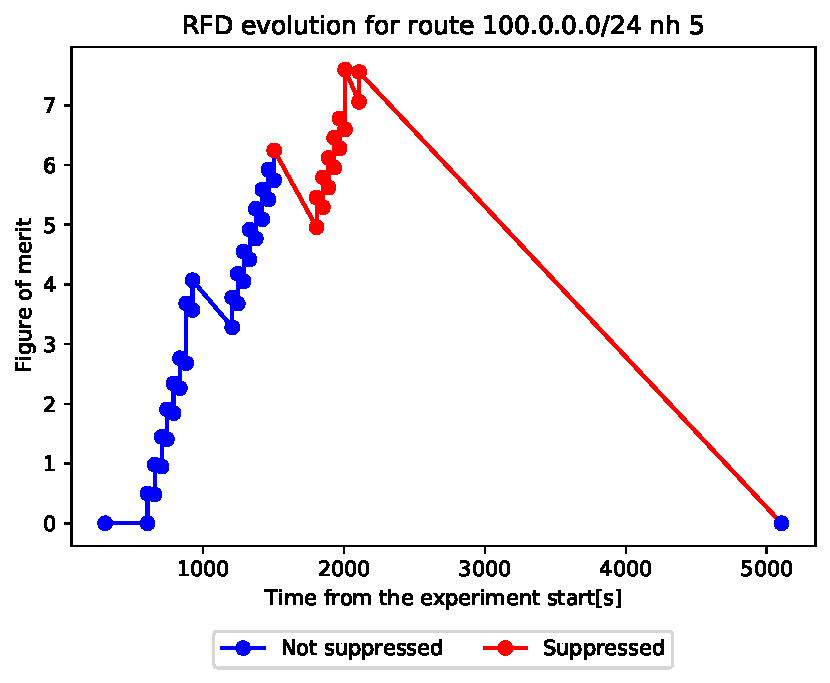
\includegraphics[width=\textwidth]{images/RFD/clique/FigureOfMerit/mrai11_RFD_7196_aggressive_x_rfd_R1.pdf}
         \caption{MRAI = 50s, RFD 7196 Aggressive, clique topology}
         \label{fig:clique_x_mrai50_rfd7196Aggressive}
     \end{subfigure}
     \hfill
     \begin{subfigure}[b]{0.3\textwidth}
         \centering
         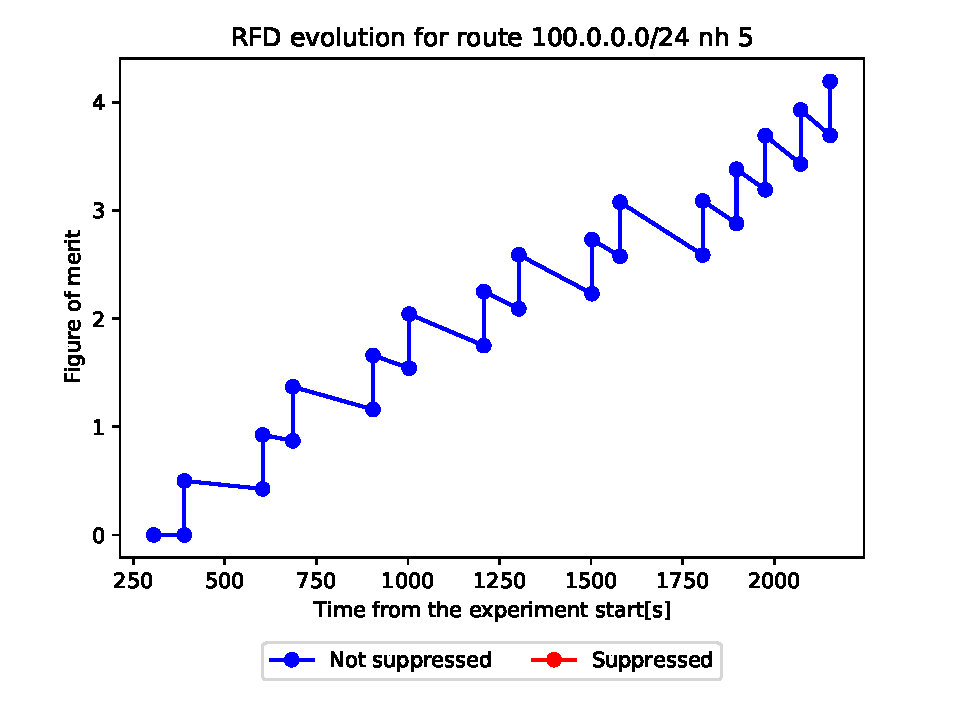
\includegraphics[width=\textwidth]{images/RFD/clique/FigureOfMerit/mrai21_RFD_7196_aggressive_x_rfd_R1.pdf}
         \caption{MRAI = 100s, RFD 7196 Aggressive, clique topology}
         \label{fig:clique_x_mrai100_rfd7196Aggressive}
     \end{subfigure}
        \caption{Evolution of the figure of merit in the node X with different MRAIs, with RFD 7196 aggressive in a clique topology}
        \label{fig:clique_nodex_rfd7196Aggressive}
\end{figure}

We can see in \Cref{fig:clique_x_mrai0_rfd7196Aggressive,fig:clique_x_mrai50_rfd7196Aggressive}
that \ac{MRAI} plays an important role in the figure of merit of node $x$.
In the first case, the route would be delayed up to \SI{4000}{\second} with a 
threshold that touches \num{12} few seconds after the first flap.
In the second one, the growth is slower but it passes the threshold around
\SI{1800}{\second} reaching a value of \num{7}.
For this reason it requires a higher time to become available again.
We can also notice that the route become available with a figure of merit of 
\num{0}, thats because it has been triggered the max suppression threshold, 
whith the defaul value of cisco after \SI{1}{\hour} a route would become available
again, no matther the evlution of the figure of merit.
With a higher \ac{MRAI} node \num{5} is able to compress more routes, the effects
are visible in \Cref{fig:clique_x_mrai100_rfd7196Aggressive}, where the figure of
merit never goes over the threshold.
 
In conclusion, if before \ac{MRAI}, with the standard \ac{RFD} was playing a more
marginal role because of the restrictive threshold, now, with those strategies
it plays a more relevant role and act as a key factor between the suppression 
or not.

%\begin{itemize}
%    \item Time comparison between both of them
%    \item how them react differently?
%    \item why?
%\end{itemize}

\section{Mice VS Elephants}
\label{sec:bgp_rfd_mice_vs_elephants}

From the work of R. Bush et al., \cite{pelsser2011route} we know that the majority
of updates that are transmitted on the Internet are from a small set of \ac{AS}.
Those \ac{AS}es with their flaps causes update storms almost continuously.
I report a figure from \cite{pelsser2011route} for simplicity in 
\Cref{fig:RBushPrefixes}
Thanks to the studies of APNIC \fxfatal{insert citation of footnote, something}
we also know that this behaviour is still present nowadays, the \Cref{fig:apnicPrefixes}
is taken from one of their annual reports and shows that the \num{10}\% of
all the active prefixes produce more or less the \num{70}\% of the total
updates.

\begin{figure}[h]
     \centering
     \begin{subfigure}[b]{0.48\textwidth}
         \centering
         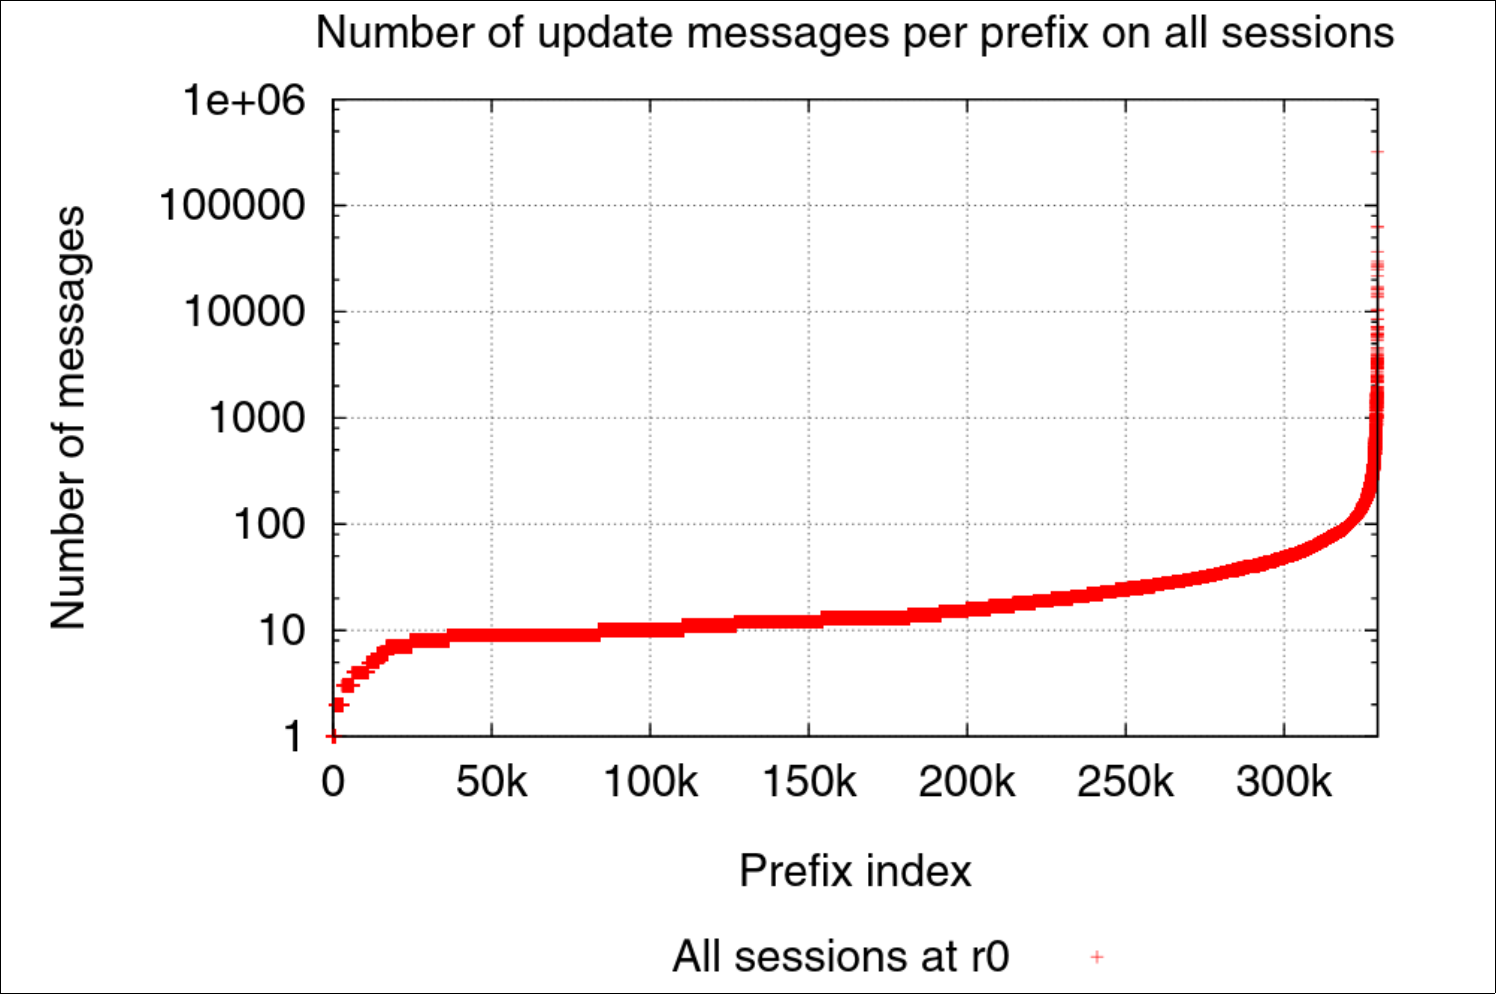
\includegraphics[width=\textwidth]{images/RFD/miceVSelephants/prefixVSmessagesRbush.png}
		 \caption{Prefixes and number of updates associated, figure from \cite{pelsser2011route}}
         \label{fig:RBushPrefixes}
     \end{subfigure}
     \hfill
     \begin{subfigure}[b]{0.48\textwidth}
         \centering
         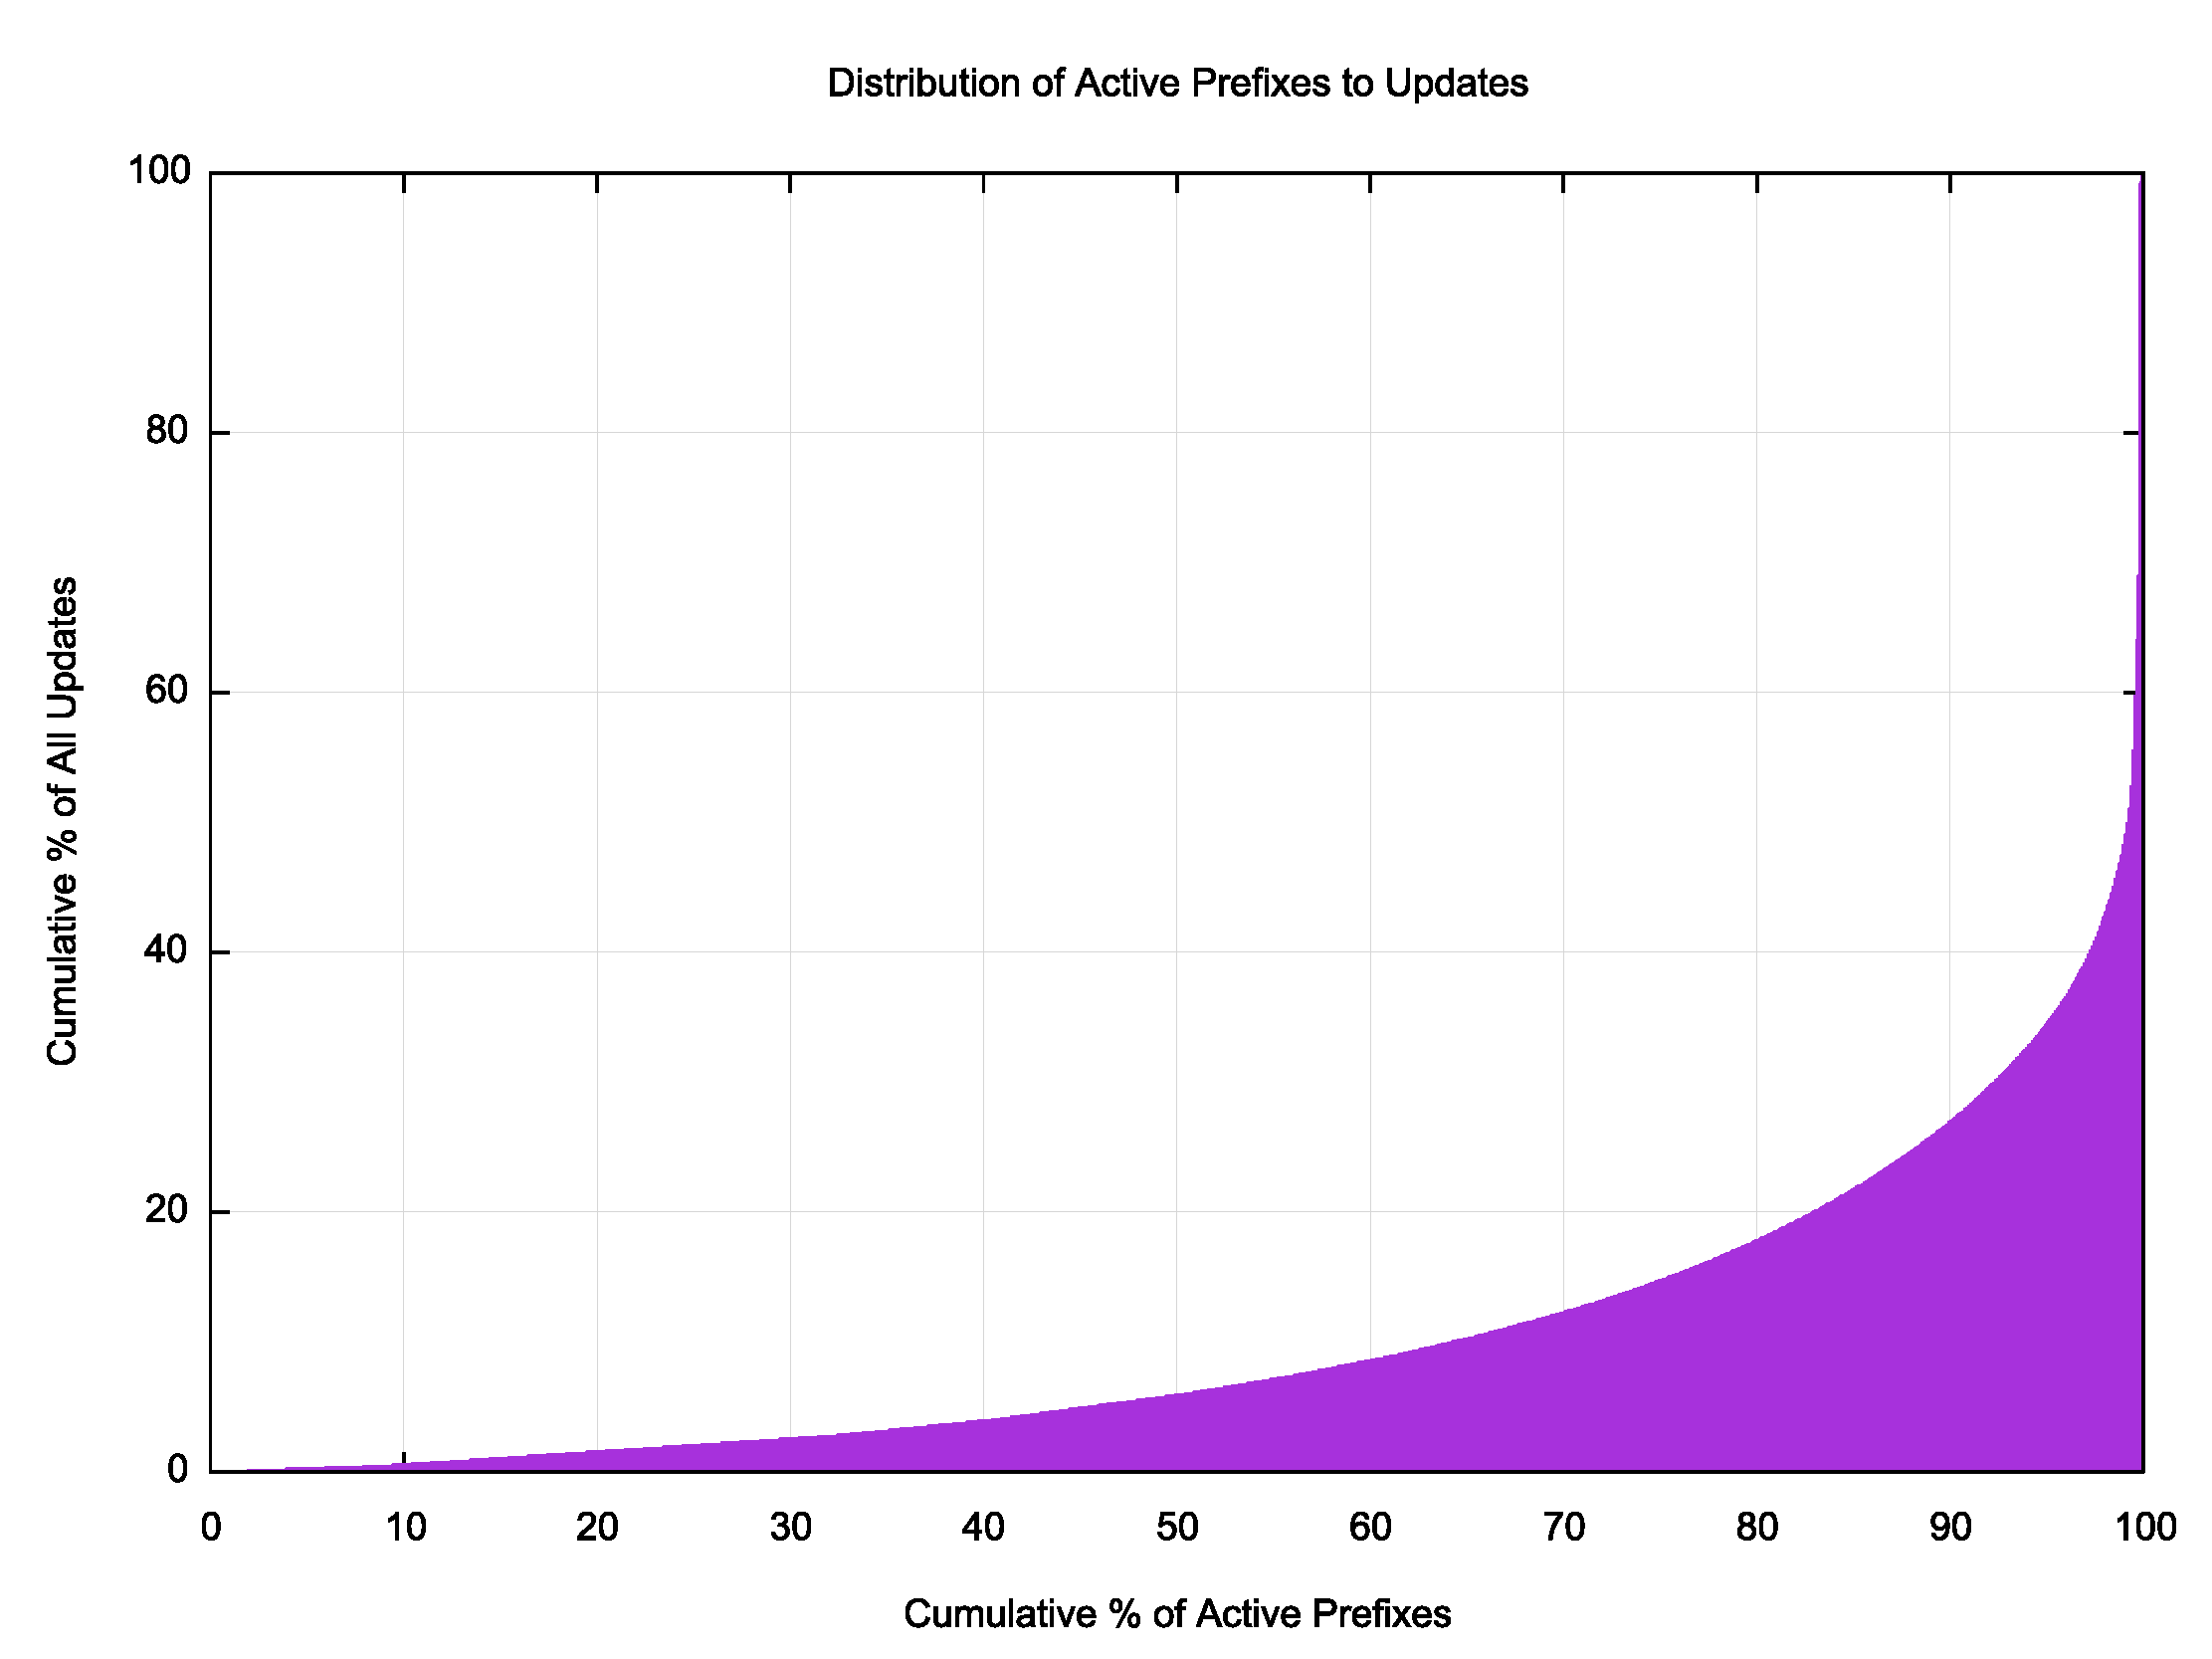
\includegraphics[width=\textwidth]{images/RFD/miceVSelephants/bgp2fig5-pfx-upds-cuml.png}
         \caption{Prefixes and number of updates associated, [apnic 2019]}
         \label{fig:apnicPrefixes}
     \end{subfigure}
        \caption{Prefixes influence on updates}
        \label{fig:prefixVSmessages}
\end{figure}

We can then divide those prefixes in two sets:
\begin{itemize}
	\item \textbf{\textit{Mice}}, this set represent the majority of the prefixes,
		all the prefixes that does not generate more than \num{100} updates 
		in \Cref{fig:RBushPrefixes}
	\item \textbf{\textit{Elephants}}, this set represent the remaining part
		of the prefixes, those that produces the majority of the messages.
\end{itemize}

Thanks to a review of a \ac{BGP} year by APNIC, presented at RIPE 52 \cite{huston2006bgp}, we can also have an example of those elephants prefixes.
This example is shown in \Cref{fig:ripePrefixFlaps}, it takes in consideration the
prefix \q{202.64.49.0/24} showing that in a relatively small period of time it has
produced thousands of \ac{ADV} per day.
In this case, this particular prefix has produced \num{198,370} \ac{ADV} producing
in total \num{96,330} flaps.

\begin{figure}[h]
    \centering
    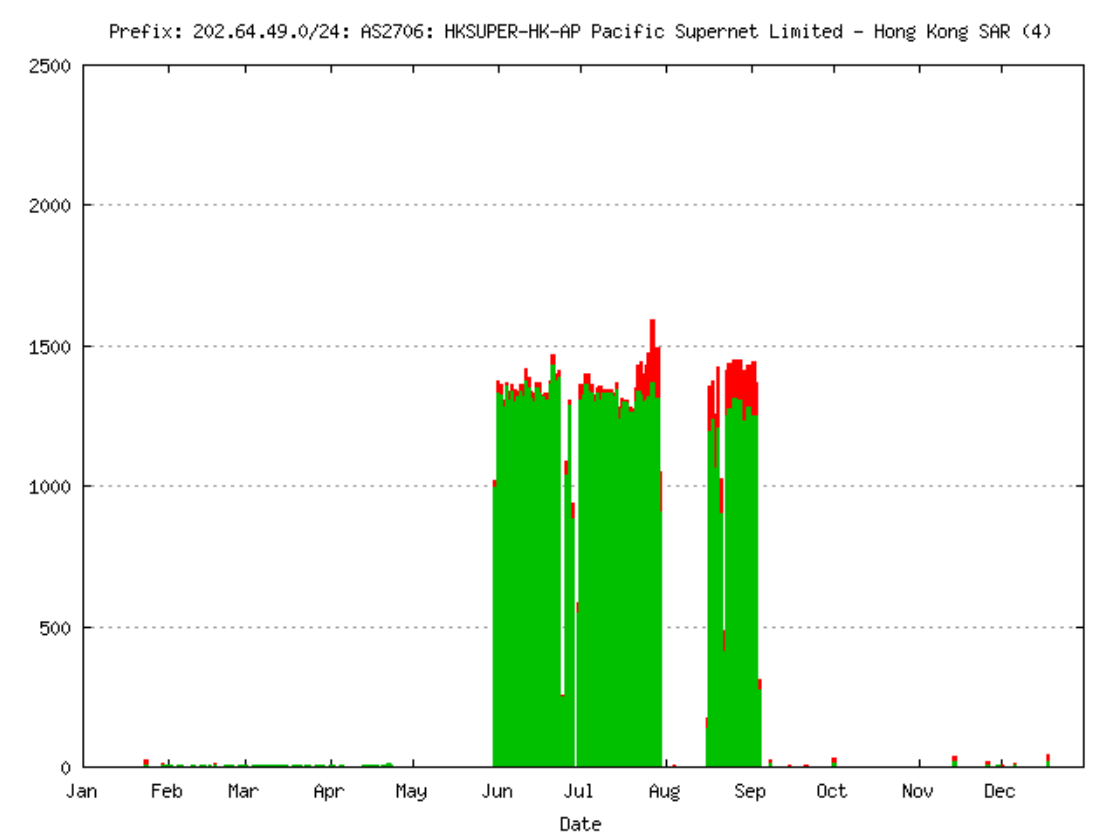
\includegraphics[scale=0.22]{images/RFD/miceVSelephants/ripePrefixFlap.png}
	\caption{202.64.49.0/24 flaps plot from \cite{huston2006bgp}}
    \label{fig:ripePrefixFlaps}
\end{figure}

I have then used this data to configure two new environments for the simulations.
The first one that points to reproduce the \textit{Mice} behaviour, the second
one the \textit{Elephants}.

In both these environments, I have then compared the four different strategies of
\ac{RFD}, \textit{NoRFD}, standard \ac{RFD} and the two from \cite{rfc7196}.

The topology used for those experiments is an \textit{Internet like} topology
with \num{1000} nodes and \ac{MRAI} is fixed to \SI{30}{\second} for all the links.
The source of the signal has been chosen randomly on the graph.
For each experiment has been then executed \num{50} runs.

\subsection{Mice}
\label{subsec:mice}

The particularity of the \textit{Mice} experiments is in the signal, we have
a low number of flaps interleaved by a long timer.
I have then used a signal with \num{5} flaps, \q{AWAWAWAWAWA} with a delay
of \SI{300}{\second} (\SI{5}{\minute}) between each message.
The results are presented in \Cref{fig:1000_RFD_MRAI30_mice}.
I have executed \num{50} runs for each \ac{RFD} strategy.

\begin{figure}[h]
     \centering
     \begin{subfigure}[b]{0.325\textwidth}
         \centering
         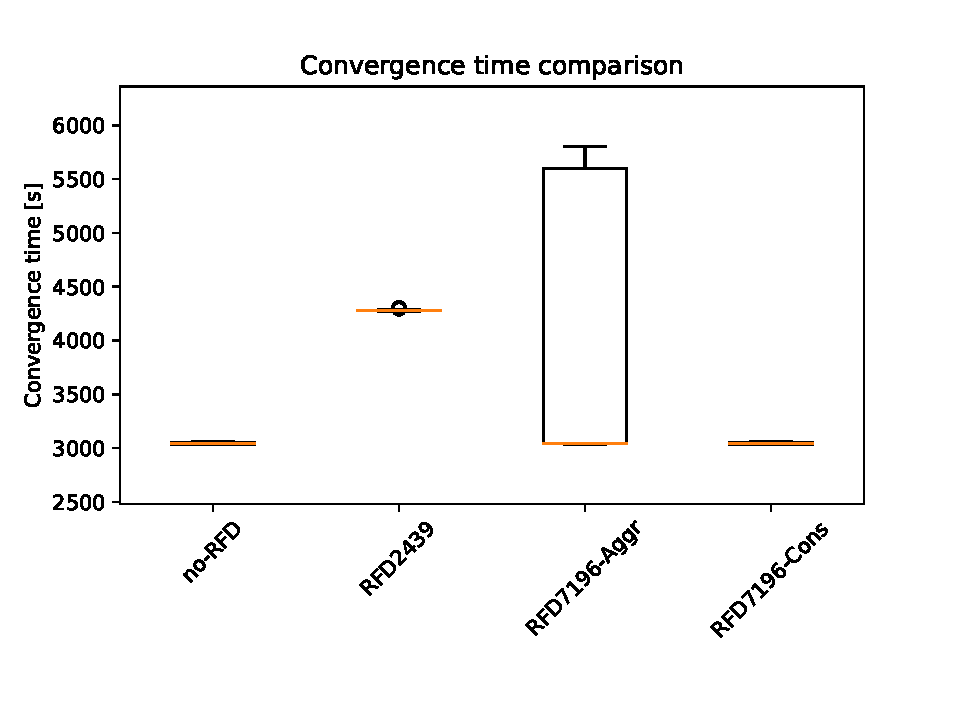
\includegraphics[width=\textwidth]{images/RFD/miceVSelephants/mice/cisco_1000MRAI30_rfd_comparison_time_boxplot.pdf}
         \caption{Convergence time respect to the RFD strategy}
         \label{fig:1000_RFD_MRAI30_mice_time}
     \end{subfigure}
     \hfill
     \begin{subfigure}[b]{0.325\textwidth}
         \centering
         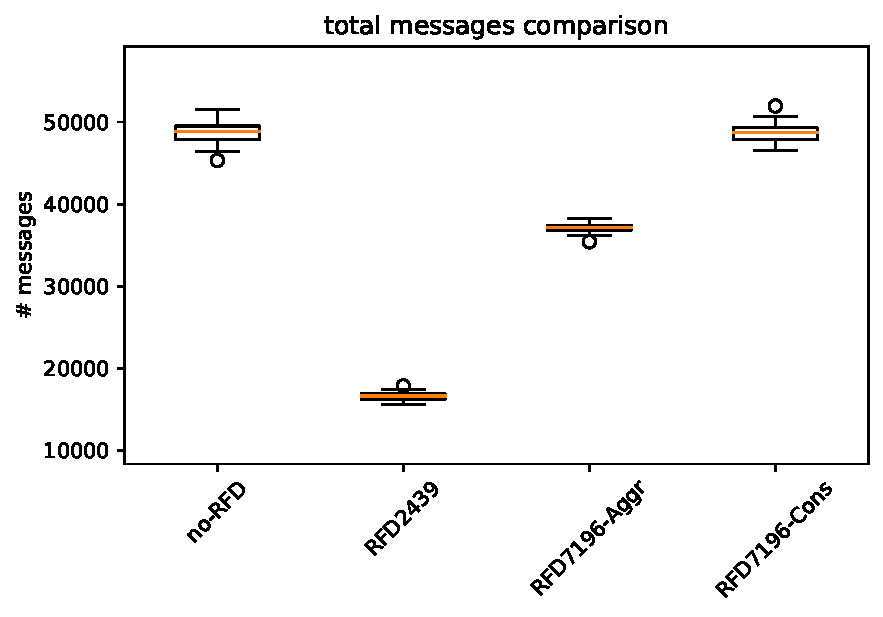
\includegraphics[width=\textwidth]{images/RFD/miceVSelephants/mice/cisco_1000MRAI30_rfd_comparison_messages_boxplot.pdf}
         \caption{Number of messages respect to the RFD strategy}
         \label{fig:1000_RFD_MRAI30_mice_messages}
     \end{subfigure}
     \hfill
     \begin{subfigure}[b]{0.325\textwidth}
         \centering
         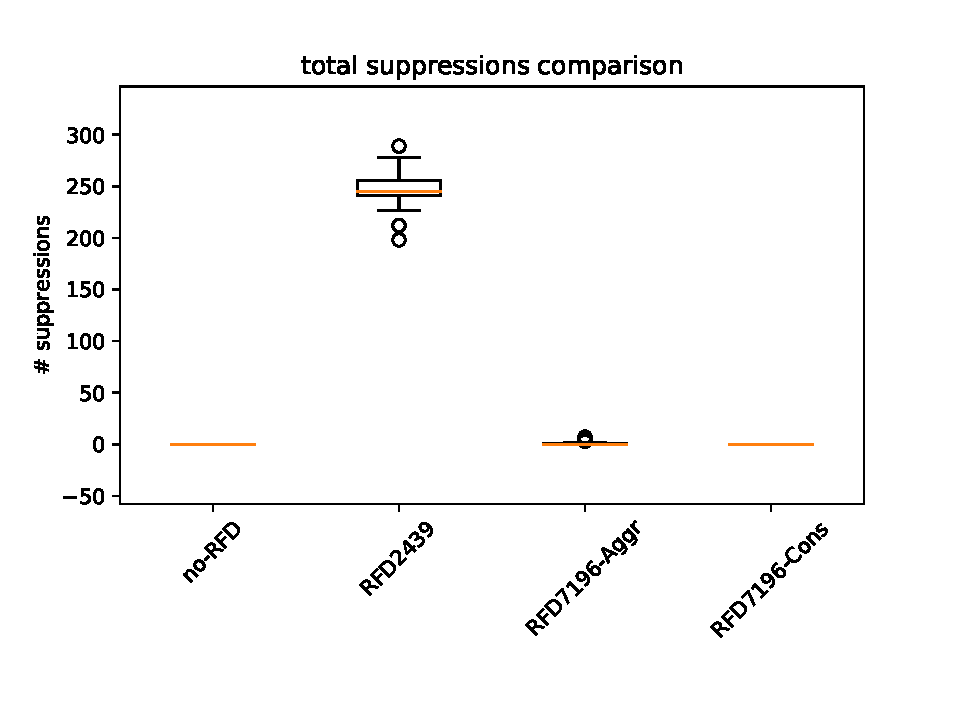
\includegraphics[width=\textwidth]{images/RFD/miceVSelephants/mice/cisco_1000MRAI30_rfd_comparison_suppressions_boxplot.pdf}
         \caption{Number of suppressions respect to the RFD strategy}
         \label{fig:1000_RFD_MRAI30_mice_suppressions}
     \end{subfigure}
		\caption{Internet like topology 1000 nodes, MRAI=30s, random destination, 
		5 flaps, \SI{300}{\second} message delay, Network performances,
		\num{50} runs per strategy.}
        \label{fig:1000_RFD_MRAI30_mice}
\end{figure}

From \Cref{fig:1000_RFD_MRAI30_mice_suppressions} we can see that there is a
big difference in terms of suppressions.
The standard strategy produces on average almost \num{1500} suppressions and the effects
of those suppressions can be seen in \Cref{fig:1000_RFD_MRAI30_mice_time,fig:1000_RFD_MRAI30_mice_messages}
because, on average, it presents a convergence time higher than \SI{6000}{\second} 
but with a number of total messages transmitted around \num{16000} with a very 
low varaiance.
A different case is presented by the \textit{Conservative} strategy from \ac{RFC}
7196 \cite{rfc7196}.
The threshold in this last case is so permessive that we have a really small 
number of suppression.
For this reason the number of messages transmitted, on average, is really similar to 
the \textit{NoRFD} case, around \num{50000}.
While, the convergence time is around \SI{6500}{\second}, like the standard \ac{RFD}
strategy.
This is prove that few suppression can heavily influence the network performances,
in particulare the convergence time.
In the middle we find the \textit{Aggressive} strategy, we can see from the
suppression boxplot that it produces a smaller number of suppressions in respect
of the legacy strategy with a smaller varaiance.
Also the nconvergence time respect this trend, infact, the average time is 
below \SI{6000}{\second}.
While, The number of messages transmitted is more than the double in respect
of the strategy described by the \ac{RFC} \num{2439}.

We can than conclude that a small number of suppression can affect both the 
performances, like the few suppressions in the \textit{Conservative} strategy
for the convergence time.
Also the few missing suppression in the \textit{Aggressive} strategy will
enormously impact the number of messages transmitted.

We can then study which are the nodes that produce the suppressions and how
far are them from the signal source.
We can see the results of this study, for each suppression technique in \Cref{fig:1000_RFD_centVSsup}.

\begin{figure}[h]
     \centering
     \begin{subfigure}[b]{0.325\textwidth}
         \centering
         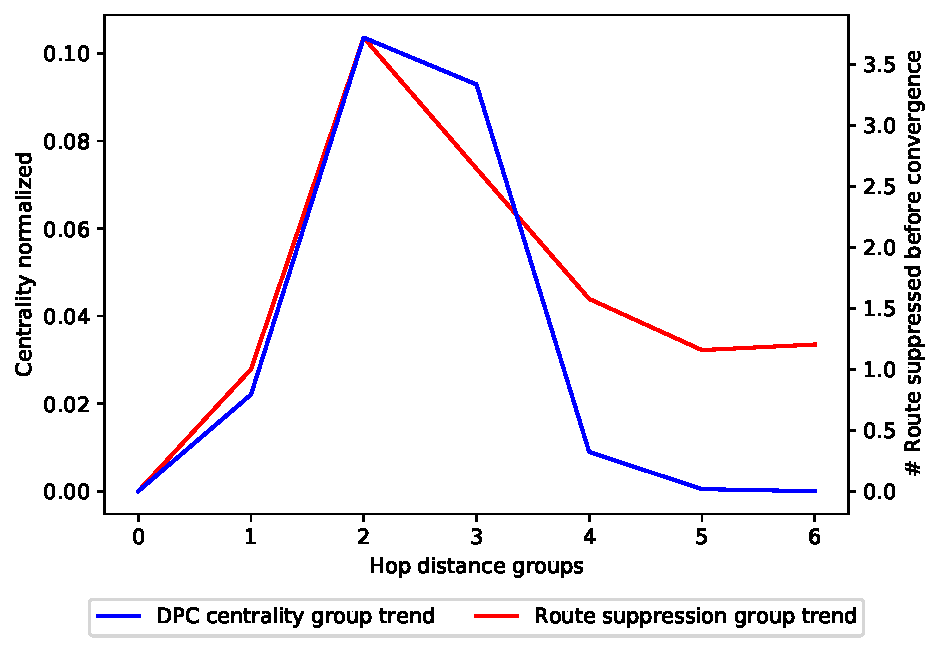
\includegraphics[width=\textwidth]{images/RFD/miceVSelephants/mice/cisco_1000_RFD_nodeConvergence_centVSsup_trend.pdf}
         \caption{RFD 2439 Strategy}
         \label{fig:1000_2439RFD_centVSsup}
     \end{subfigure}
     \hfill
     \begin{subfigure}[b]{0.325\textwidth}
         \centering
         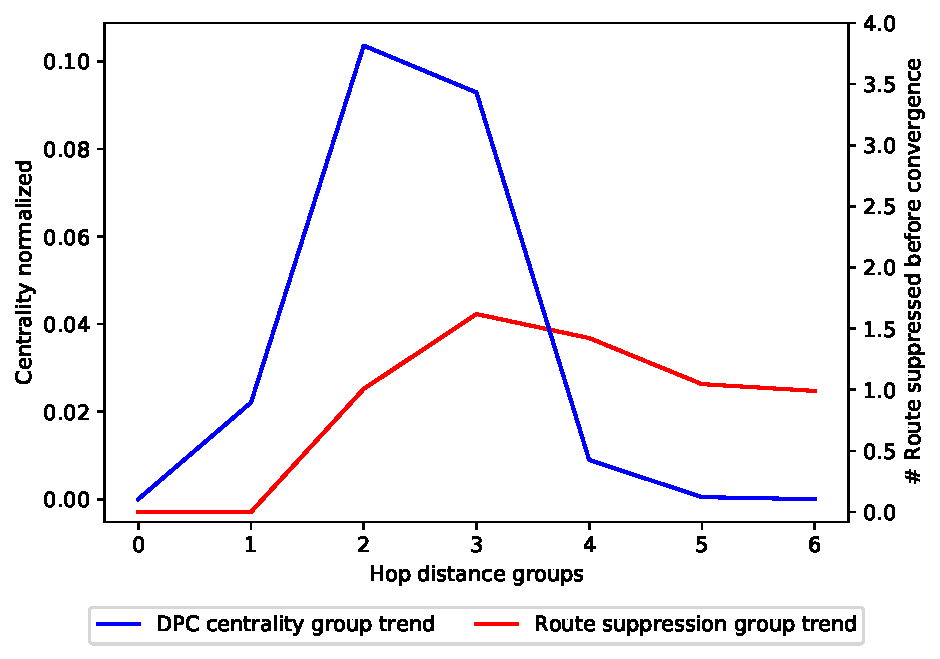
\includegraphics[width=\textwidth]{images/RFD/miceVSelephants/mice/cisco_1000_RFD_7196_aggressive_nodeConvergence_centVSsup_trend.pdf}
         \caption{RFD 7196 Aggressive Strategy}
         \label{fig:1000_7196RFDA_centVSsup}
     \end{subfigure}
     \hfill
     \begin{subfigure}[b]{0.325\textwidth}
         \centering
         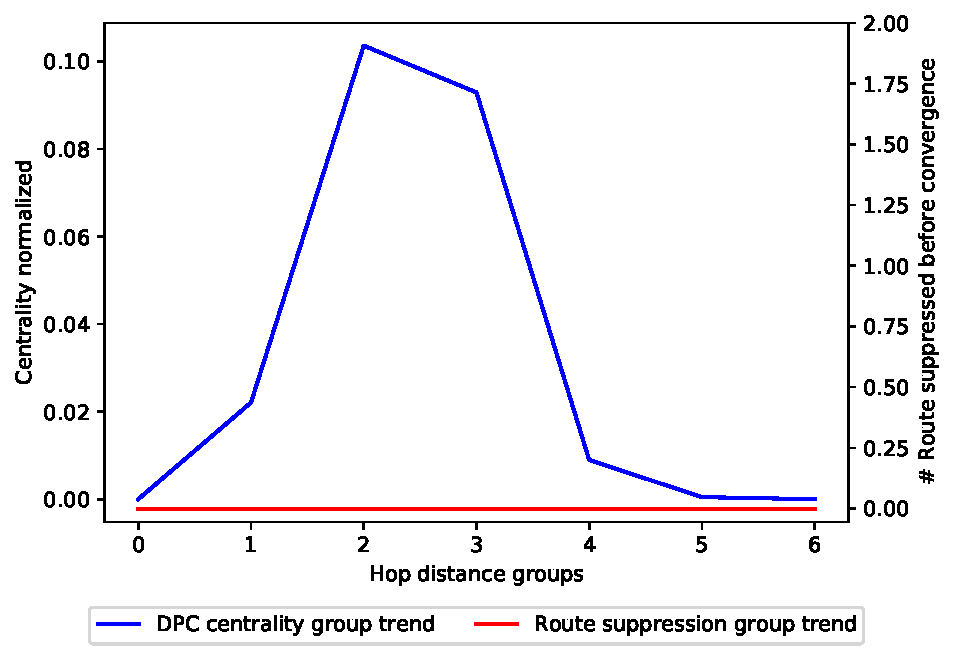
\includegraphics[width=\textwidth]{images/RFD/miceVSelephants/mice/cisco_1000_RFD_7196_conservative_nodeConvergence_centVSsup_trend.pdf}
         \caption{RFD 7196 Conservative Strategy}
         \label{fig:1000_7196RFDC_centVSsup}
     \end{subfigure}
		\caption{Internet like topology \num{1000} nodes, \ac{MRAI} = \SI{30}{\second}, random destination, \num{5} flaps, \SI{300}{\second} between messages, Suppression trend VS avg hop centrality}
        \label{fig:1000_RFD_centVSsup}
\end{figure}

\fxfatal{Adjust the y-axis}

For the plots in \Cref{fig:1000_RFD_centVSsup} the $x$ axis represent the distance
from the source node in terms of hops and all the other nodes are grouped by this
distance.
The blue line represents the average centrality of the groups, for each node of the
graph I calculated the centrality using the \ac{DPC} metric then grouped them
and calculated the average value.
As expected the central nodes have a higher centrality and them are at few hops
of distance
from the source node.
The centrality trend is equal for each plot in \Cref{fig:1000_RFD_centVSsup}
because the graph and the source node are the same for each experiment.

The red line represents the average number of suppressions per group.
As we can see with the standard strategy, \Cref{fig:1000_2439RFD_centVSsup}, 
on average, the route is blocked \num{1} time by the nearest nodes and then, 
this value increase reaching the center clique up to \num{3.5} times and then
slowly decreases in the following groups.
In the farest group we will still see, on average \num{1} suppression.
The \textit{Aggressive} strategy, \Cref{fig:1000_7196RFDA_centVSsup} present
a similar behaviour, the nearest nodes don't blocks the route, while the central
nodes starts blocking it with a maximum average of \num{1.6} times.
Aftter those central nodes, the farest nodes, that have a low entrality will
block it on average \num{1} time, like the legacy strategy.
The \textit{Conservative} strategy, presented in \Cref{fig:1000_7196RFDC_centVSsup},
has a different trend.
We can see that the central nodes does not block the route, while only the farest
ones blocks it few times, with an average value of \num{0.2} times.
This can gives us some hints, a very high threshold can promote the path
exploration problem that will cause multiple update storms in farest nodes.

\fxfatal{Add a conclusion}

\subsection{Elephants}
\label{subsec:bgp_elephants}

The elephants prefixes, as I mentioned in \Cref{sec:bgp_rfd_mice_vs_elephants},
are the ones that produce the majority of the \ac{ADV}.
And we also know, thanks to \cite{huston2006bgp}, that is possible to see over
thousands of messages per day.
For this reason, the \textit{elephants} environment signal is composed by \num{100}
flaps, with a delay between the messages of \SI{3}{\second}.
All the other properties of the environment are unchanged.
The results are presented in \Cref{fig:1000_RFD_MRAI_30_elephant,fig:1000_RFD_cent_VS_sup_elephants}.

\begin{figure}[h]
     \centering
     \begin{subfigure}[b]{0.325\textwidth}
         \centering
         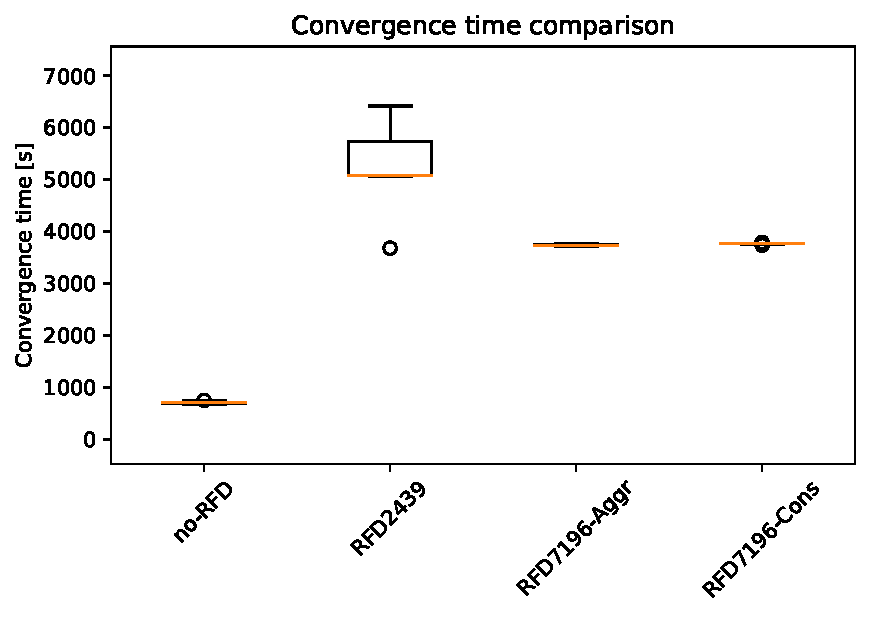
\includegraphics[width=\textwidth]{images/RFD/miceVSelephants/elephants/cisco_1000MRAI30_rfd_comparison_time_boxplot.pdf}
         \caption{Convergence time respect to the RFD strategy}
         \label{fig:1000_RFD_MRAI_30_time_elephant}
     \end{subfigure}
     \hfill
     \begin{subfigure}[b]{0.325\textwidth}
         \centering
         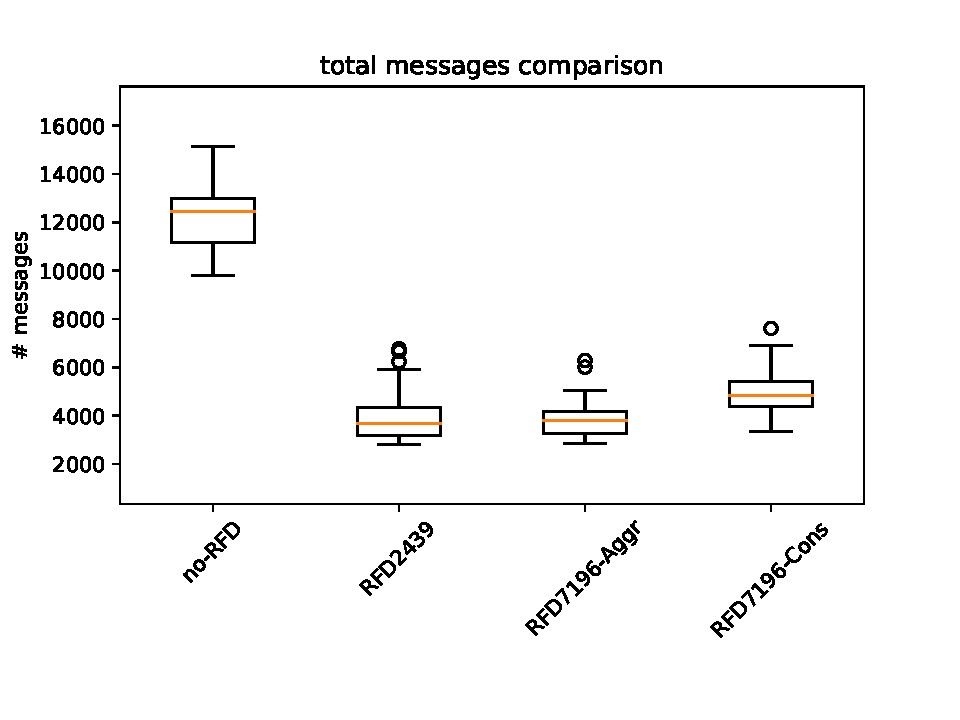
\includegraphics[width=\textwidth]{images/RFD/miceVSelephants/elephants/cisco_1000MRAI30_rfd_comparison_messages_boxplot.pdf}
         \caption{Number of messages respect to the RFD strategy}
         \label{fig:1000_RFD_MRAI_30_messages_elephant}
     \end{subfigure}
     \hfill
     \begin{subfigure}[b]{0.325\textwidth}
         \centering
         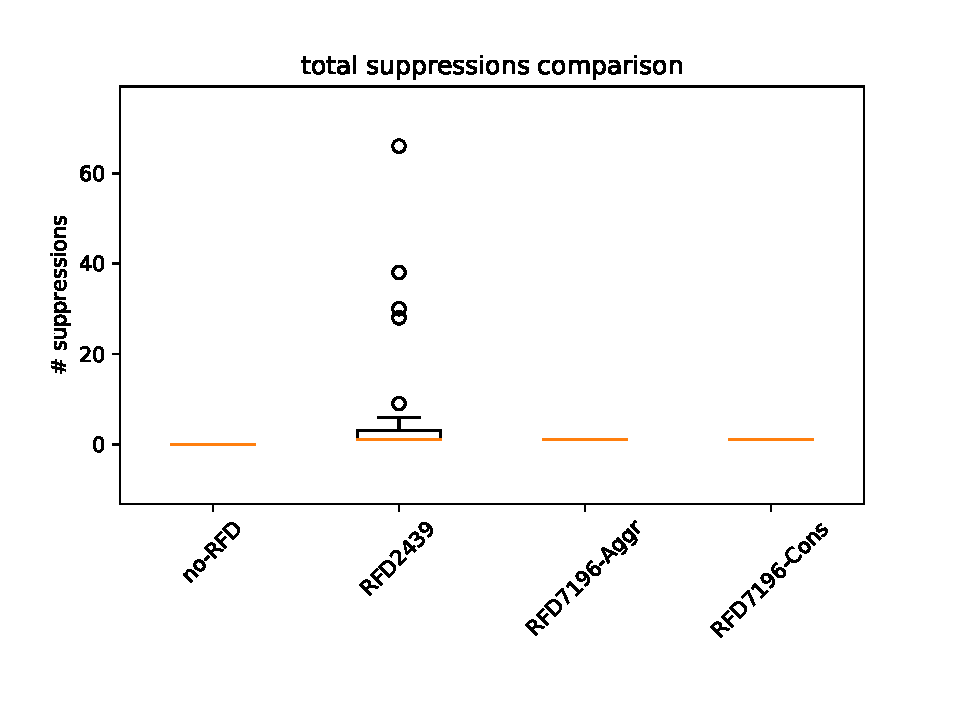
\includegraphics[width=\textwidth]{images/RFD/miceVSelephants/elephants/cisco_1000MRAI30_rfd_comparison_suppressions_boxplot.pdf}
         \caption{Number of suppressions respect to the RFD strategy}
         \label{fig:1000_RFD_MRAI_30_suppressions_elephant}
     \end{subfigure}
		\caption{Internet like topology \num{1000} nodes, \ac{MRAI} = \SI{30}{\second}, random destination, \num{100} flaps, \SI{3}{\second} delay, Network performances}
        \label{fig:1000_RFD_MRAI_30_elephant}
\end{figure}

Is possible to see in \Cref{fig:1000_RFD_MRAI_30_elephant} that this time we have
a different behaviour from all the \num{3} \ac{RFD} strategies.
In \Cref{fig:1000_RFD_MRAI_30_suppressions_elephant} we can see that the
The standard strategy does more than \num{1250} suppression on average, producing 
the lowest number of messages, around \num{11000} but the highest convergence
time with more than \SI{5000}{\second}.
All the suppression are trigger by the \textit{Path Exploration} problem that 
causes repitetvly \ac{ADV} storms that trigger the suppressions on the majority
of the nodes.
The two new strategies would produce on average just few suppressions in respect
of the legacy one, but the number of messages doesn't differ too much.
While there is a huge improvement on the convergence time, on average,
both the new strategy permits to the network to converge in less than \SI{4000}{\second}.
All the three strategy produce $1/3$ of the messages produced by the 
\textit{NoRFD} strategy.

\begin{figure}[h]
     \centering
     \begin{subfigure}[b]{0.325\textwidth}
         \centering
         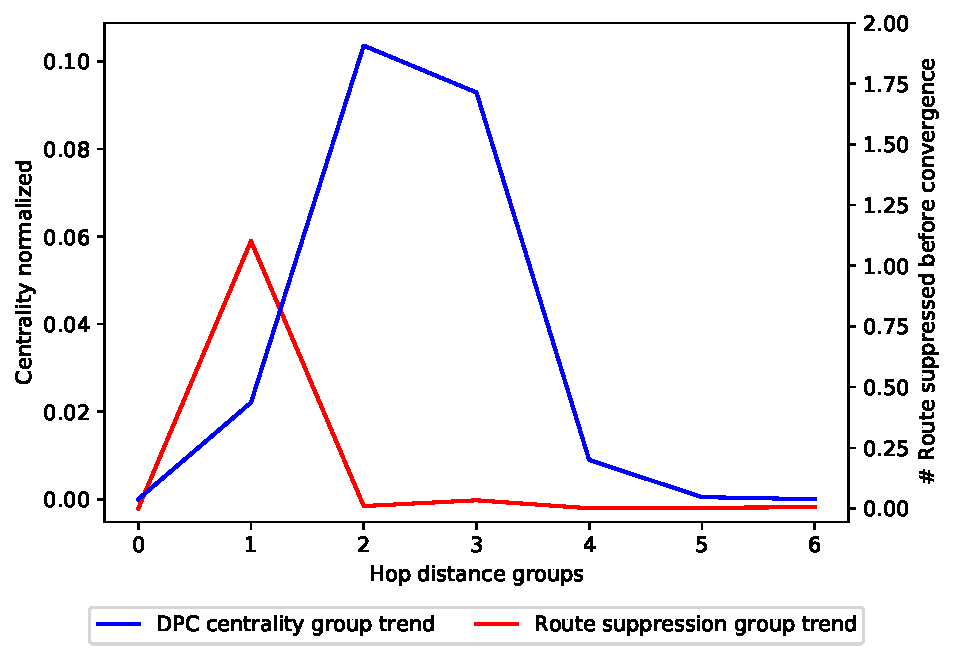
\includegraphics[width=\textwidth]{images/RFD/miceVSelephants/elephants/cisco_1000_RFD_nodeConvergence_centVSsup_trend.pdf}
         \caption{RFD 2439 Strategy}
         \label{fig:1000_2439RFD_cent_VS_sup_elephants}
     \end{subfigure}
     \hfill
     \begin{subfigure}[b]{0.325\textwidth}
         \centering
         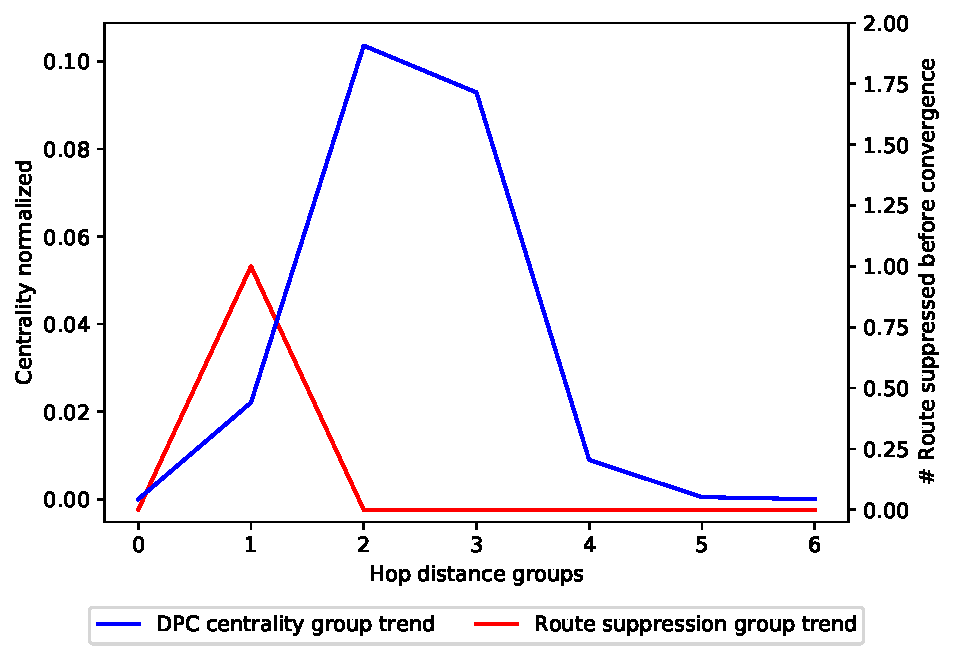
\includegraphics[width=\textwidth]{images/RFD/miceVSelephants/elephants/cisco_1000_RFD_7196_aggressive_nodeConvergence_centVSsup_trend.pdf}
         \caption{RFD 7196 Aggressive Strategy}
         \label{fig:1000_7196RFDA_cent_VS_sup_elephants}
     \end{subfigure}
     \hfill
     \begin{subfigure}[b]{0.325\textwidth}
         \centering
         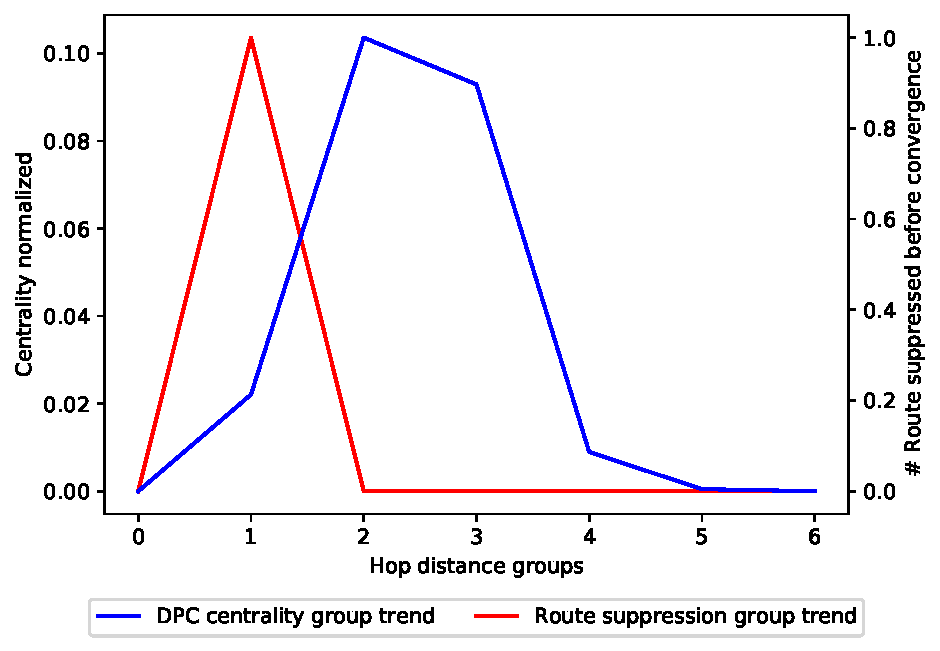
\includegraphics[width=\textwidth]{images/RFD/miceVSelephants/elephants/cisco_1000_RFD_7196_conservative_nodeConvergence_centVSsup_trend.pdf}
         \caption{RFD 7196 Conservative Strategy}
         \label{fig:1000_7196RFDC_cent_VS_sup_elephants}
     \end{subfigure}
		\caption{Internet like topology \num{1000} nodes, \ac{MRAI} = \SI{30}{\second}, 
		random destination, \num{100} flaps, \SI{3}{\second} delay, suppressions 
		by distance from the source}
        \label{fig:1000_RFD_cent_VS_sup_elephants}
\end{figure}

We can see in \Cref{fig:1000_RFD_cent_VS_sup_elephants} the comparison between
the average number of suppressions per node group of the different strategies.
In \Cref{fig:1000_7196RFDA_cent_VS_sup_elephants,fig:1000_7196RFDC_cent_VS_sup_elephants}
we can notice that both strategies reacts in the exact same way at the elephant
environment.
The only nodes that suppress the route are the nodes that are closer to the source.
All the other nodes of the network doesn't experience enough messages to block 
the route.
In the first figure, \Cref{fig:1000_2439RFD_cent_VS_sup_elephants}, we can see
that, on average, every node suppress at least one time the source of the
signal.
The hipothesis behind this trend is that the intervention of the closer nodes
is not timely enough and all the other nodes have the time to experience the
path exploration problem.
With a low threshold is sufficient a small number of \ac{ADV} storms caused
by the \textit{Path Exploration} to trigger the \ac{RFD} suppression.

%We can then say that all the strategies catch in time the flap and avoid the
%propagation of the update storm, increasing the convergence time but protecting 
%the network from thousands of messages.
\fxfatal{Ri-elaborate the end of the subsection}

\subsection{MRAI influence on Mice and Elephants}
\label{subsec:bgp_rfd_mrai_influence_mice_elephants}

We can now study the influence of \ac{MRAI} on those two cases.
The environments are equal to the previous section.
The results of the \textit{Mice} case are exposed in \Cref{fig:1000_RFD_multiMRAI_mice},
while the results of the elephant case are in \Cref{fig:1000_RFD_multiMRAI_elephants}.

\begin{figure}[h]
     \centering
     \begin{subfigure}[b]{0.325\textwidth}
         \centering
         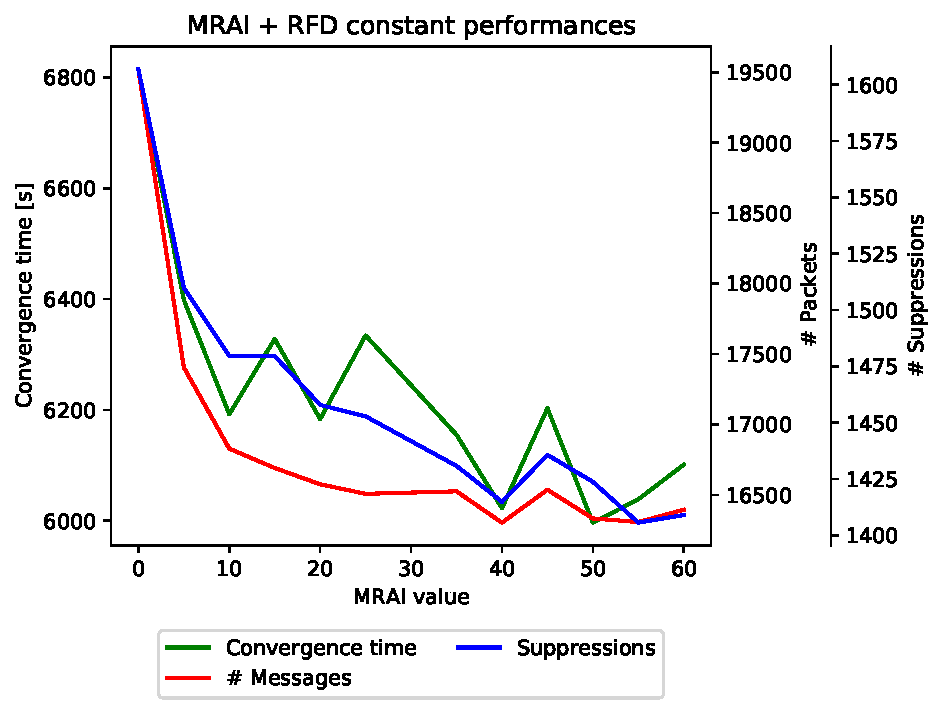
\includegraphics[width=\textwidth]{images/RFD/miceVSelephants/MultiMRAI/mice/cisco_1000_RFD_2439-constant_mrai_rfd_evolution.pdf}
         \caption{RFD 2439 Strategy}
         \label{fig:1000_2439RFD_multiMRAI_mice}
     \end{subfigure}
     \hfill
     \begin{subfigure}[b]{0.325\textwidth}
         \centering
         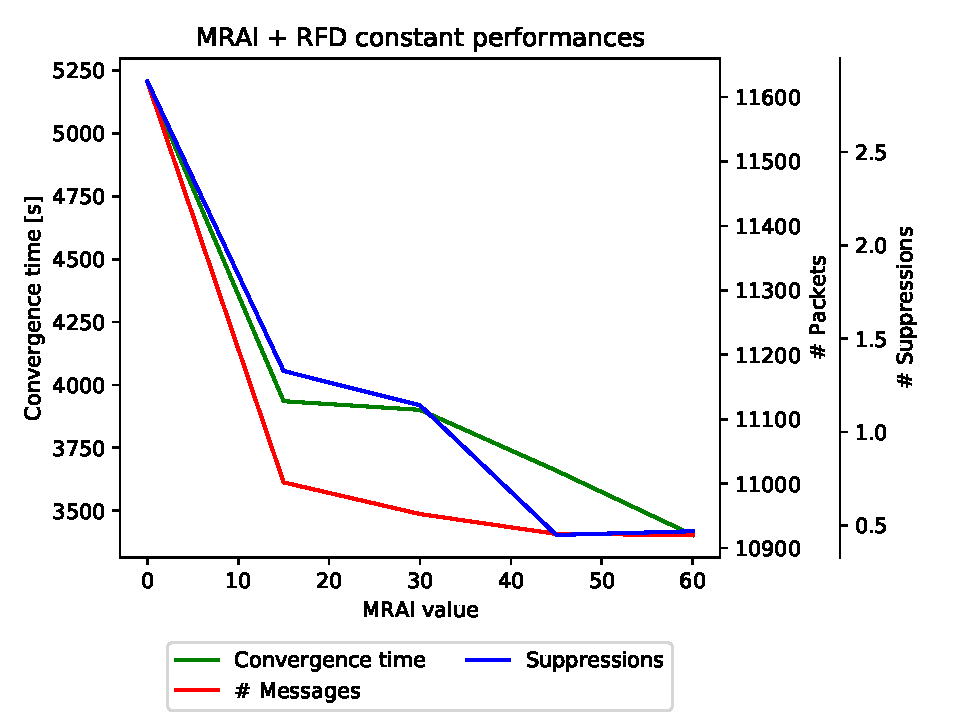
\includegraphics[width=\textwidth]{images/RFD/miceVSelephants/MultiMRAI/mice/cisco_1000_RFD_7196_aggressive-constant_mrai_rfd_evolution.pdf}
         \caption{RFD 7196 Aggressive Strategy}
         \label{fig:1000_7196RFDA_multiMRAI_mice}
     \end{subfigure}
     \hfill
     \begin{subfigure}[b]{0.325\textwidth}
         \centering
         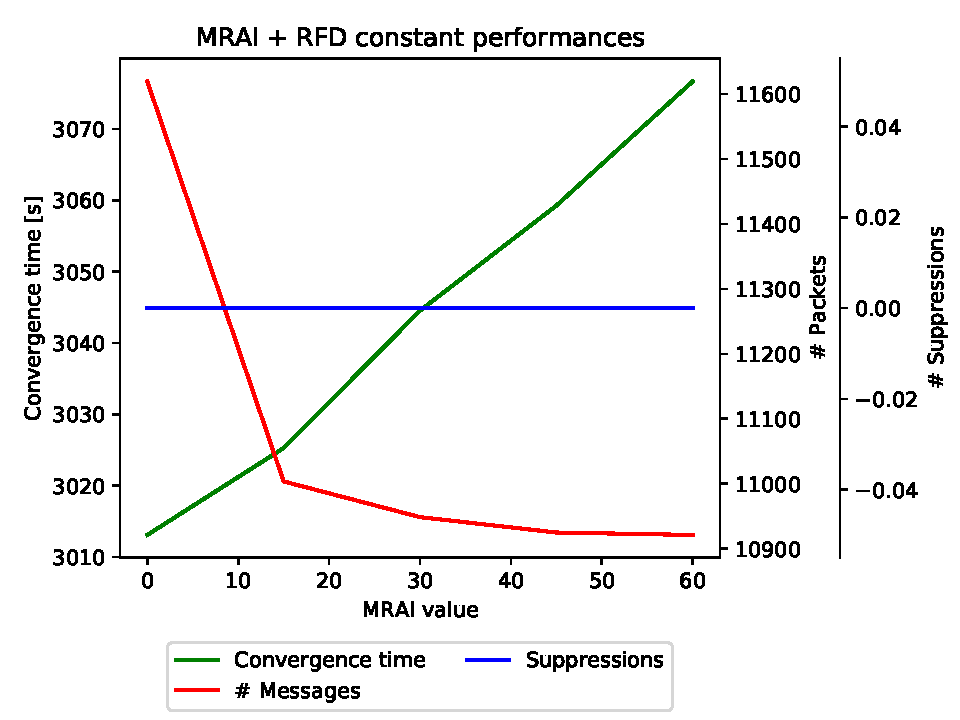
\includegraphics[width=\textwidth]{images/RFD/miceVSelephants/MultiMRAI/mice/cisco_1000_RFD_7196_conservative-constant_mrai_rfd_evolution.pdf}
         \caption{RFD 7196 Conservative Strategy}
         \label{fig:1000_7196RFDC_multiMRAI_mice}
     \end{subfigure}
		\caption{Internet like topology \num{1000} nodes, random destination, 
		\num{5} flaps, \SI{300}{\second} delay, Network performances, \ac{MRAI}
		strategy fixed}
        \label{fig:1000_RFD_multiMRAI_mice}
\end{figure}

\fxfatal{Redo this graphs with more \ac{MRAI} values, update the figures with the same y-range}

We can see in \Cref{fig:1000_RFD_multiMRAI_mice} how the different \ac{RFD} strategies
reacts, on the same topology, whith different \ac{MRAI} settings.
In \Cref{fig:1000_2439RFD_multiMRAI_mice} are presented the network performances
with the legacy \ac{RFD} strategy from the \ac{RFC} \num{2439} \cite{rfc2439}.
First of all we can see the influence of \ac{MRAI} on the number of suppressions
that decrease from \num{1600} with an \ac{MRAI} equal to \SI{0}{\second} to almost
\num{1400} with \ac{MRAI} $=$ \SI{60}{\second}.
We can notice that the message trend reacts as expected with the increasing of
\ac{MRAI}, but its noticeable that with an \ac{MRAI} of \SI{0}{\second} there
are less than \num{20000} messages thanks to \ac{RFD}.
The convergence time doesn't have the same trend as other \ac{MRAI} experiments,
it has a decreasing trend, while we were expecting an increasing one.
This is caused by the routes that doesn't suppress anymore the route.
It is greater the gain obtained by the suppression reduction than the disadvantage
caused by \ac{MRAI} that requires to the node to wait mroe time.

The second case we can analyze is the \textit{Aggressive} strategy presented
in \Cref{fig:1000_7196RFDA_multiMRAI_mice}.
We can easily notice that this time the variation in terms of suppression is smaller,
going from a value of \num{1265} to \num{1240} suppressions.
The number of messages has a similar trend to the standard strategy, but whith
a different range.
At the beginning, with \ac{MRAI} $=$ \SI{0}{\second} there are more than \num{42000}
messages, after a while it converges around a value of \num{37000} messages.
The convergence time has the expected trend by the growth of \ac{MRAI}.
The number of messages higher is caused by the fact that \ac{RFD} requires more time
to activate itself, and in the meanwhile a lot of messages storm will pass the
network.
The convergence time, in this case is not affected by the decrease of the number
of suppressions.
The gain obtained by the \ac{RFD} suppressions trend doesn't compensate the 
effects of \ac{MRAI} that makes the convergence time grow.

In the last strategy, the \textit{Conservative} one, we can see an other, different
behaviour.
In terms of suppressions \ac{MRAI} makes a huge difference, we go from \num{1200}
suppressions to \num{0} and just an \ac{MRAI} of \SI{15}{\second} reduce it around
\num{50}.
Also in this case the number of messages are higher than the other two strategies.
Like before for the \textit{Aggressive} strategy this is caused by the not
restrictive thresholds.
An interesting behaviour can be seen for the convergence time, infact like for
the \textit{Aggressive} strategy it starts grwoing also with more than \num{1000}
suppressions of difference, but as soon the number of suppression tuches \num{0}
it goes back to the \textit{NoRFD} behaviour.

All this comparison can be also seen in \Cref{fig:1000_RFD_MRAI30_mice,fig:1000_RFD_centVSsup_mices}.

\Cref{fig:1000_2439RFD_multiMRAI_mice} compared with \Cref{fig:1000_7196RFDA_multiMRAI_mice}
tels us that not all the gain in terms of suppressions gives also advantages in 
termes con convergence time.
\fxfatal{Not sure of this phrase, it could be due to the threshold}.
Also a difference of few hundred suppression have a huge impact in the messages
transitted.

In \Cref{fig:1000_RFD_multiMRAI_elephants} are presented the results obtained
with the elephant environment and multiple \ac{MRAI} values.

\begin{figure}[h]
     \centering
     \begin{subfigure}[b]{0.325\textwidth}
         \centering
         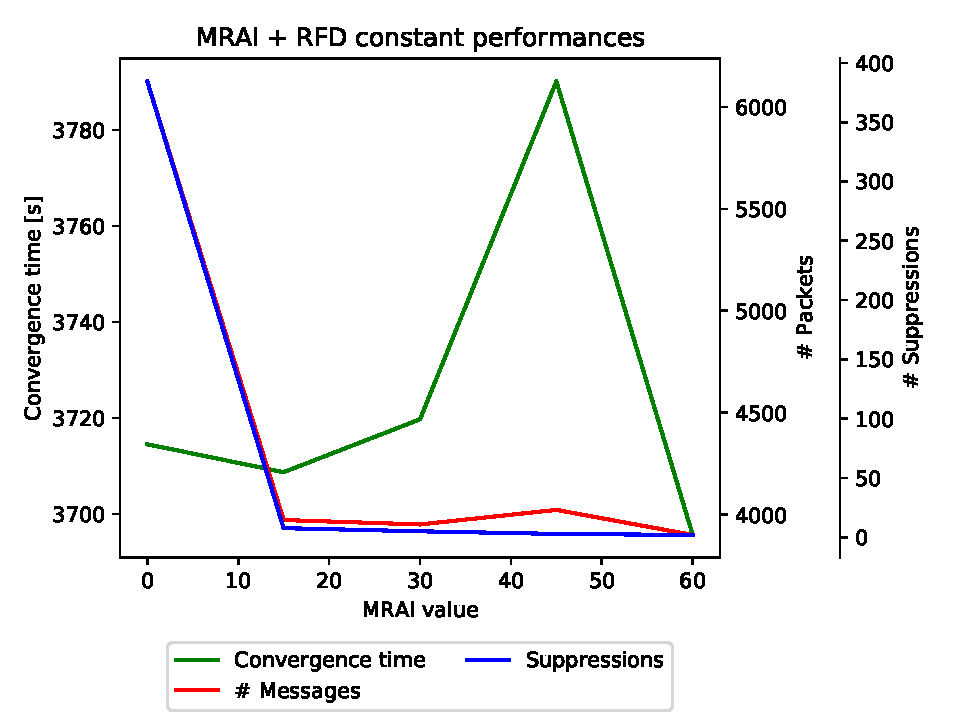
\includegraphics[width=\textwidth]{images/RFD/miceVSelephants/MultiMRAI/elephants/cisco_1000_RFD_2439-constant_mrai_rfd_evolution.pdf}
         \caption{RFD 2439 Strategy}
         \label{fig:1000_2439RFD_multiMRAI_elephants}
     \end{subfigure}
     \hfill
     \begin{subfigure}[b]{0.325\textwidth}
         \centering
         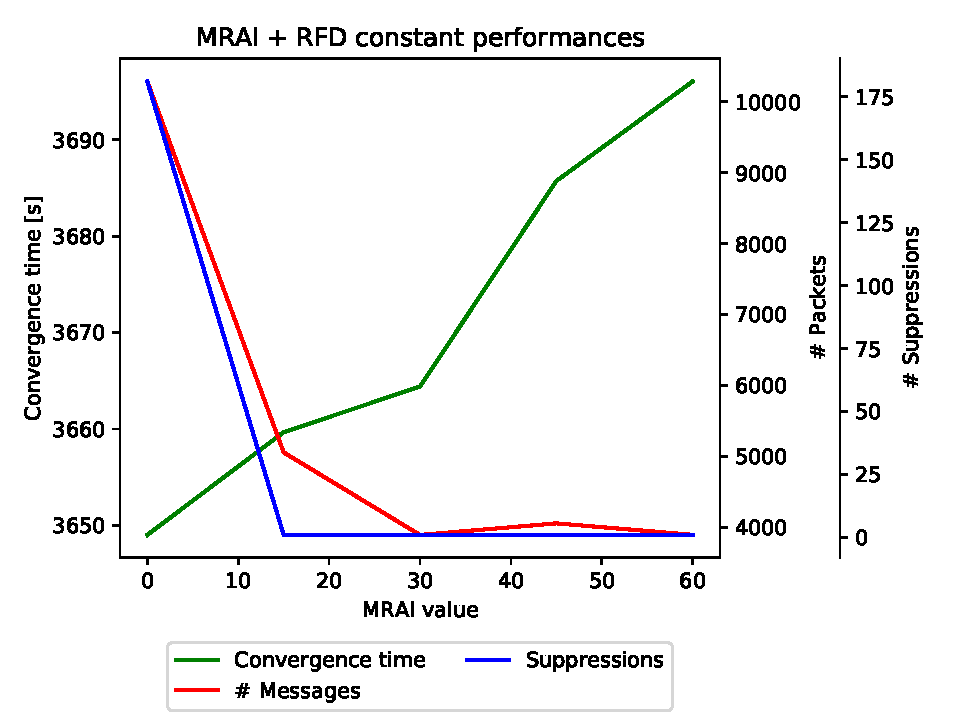
\includegraphics[width=\textwidth]{images/RFD/miceVSelephants/MultiMRAI/elephants/cisco_1000_RFD_7196_aggressive-constant_mrai_rfd_evolution.pdf}
         \caption{RFD 7196 Aggressive Strategy}
         \label{fig:1000_7196RFDA_multiMRAI_elephants}
     \end{subfigure}
     \hfill
     \begin{subfigure}[b]{0.325\textwidth}
         \centering
         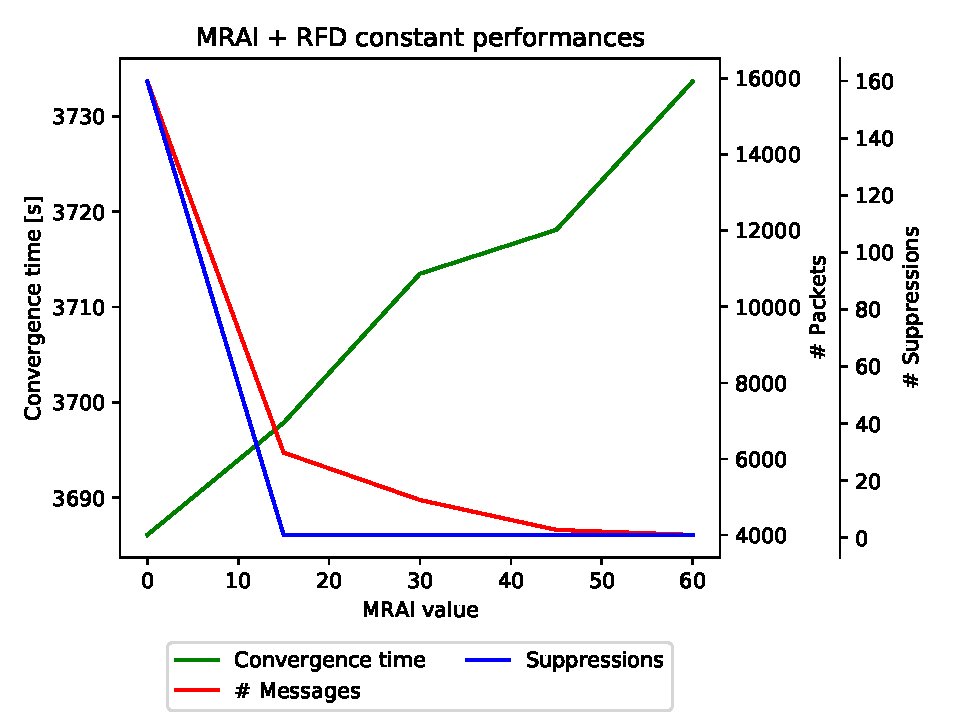
\includegraphics[width=\textwidth]{images/RFD/miceVSelephants/MultiMRAI/elephants/cisco_1000_RFD_7196_conservative-constant_mrai_rfd_evolution.pdf}
         \caption{RFD 7196 Conservative Strategy}
         \label{fig:1000_7196RFDC_multiMRAI_elephants}
     \end{subfigure}
		\caption{Internet like topology \num{1000} nodes, random destination, \num{100} flaps, \SI{3}{\second} delay, Network performances}
        \label{fig:1000_RFD_multiMRAI_elephants}
\end{figure}

The trends in the elephant case are compleatly different in respect of the
mice environment.
Starting from the standard strategy in \Cref{fig:1000_2439RFD_multiMRAI_mice}
we can see that the number of suppressions decreases of few hundred units
thanks to a higher \ac{MRAI}.
Also the number of messages decrease from around \num{14500} reaching a stable
state around \num{11000}.
While the convergence time benefits of the suppression rate decrease reaching 
a valley around \SI{5400}{\second}. 
But, after that point the effect of the next suppressions is not enough to keep
a descending trend, while \ac{MRAI} acquire a more predominant position making
the convergence time slightly increasing.
A different behaviour can be saw in 
\Cref{fig:1000_7196RFDA_multiMRAI_elephants,fig:1000_7196RFDC_multiMRAI_elephants},
where, the number off suppressions thanks to \ac{MRAI} reaches a number slightly
higher than \num{0}.
The number of messages reaches the same convergence point around \num{12500} but
with a compleatly different starting point.
with \ac{MRAI} at \SI{0}{\second} the aggressive strategy present a number of 
messages around \num{32500} while the conservative strategy is around \num{60000},
almost the double of the \textit{Aggressive} one.
This huge difference is caused by the fact that the conservative strategy requires
more flaps to overcome the suppressioon threshold, and all those messages can 
cause a more and more updates storms, due to the \textit{Path exploration} problem
in the other parts of the network.
In both, \textit{Aggressive} and \textit{Conservative} strategy the convergence
time is not affected by the variation on the number of suppressions but it's only
affected by the growth of \ac{MRAI}.

The fact that in the last two strategies the time is not affected by the huge number
of suppressions difference could be saw as an error, but it is not.
In fact, the suppressions with an \ac{MRAI} of \SI{0}{\second} happens
few seconds after the beginning of the experiment and the majority of the nodes
will suppress the route, but we know that after \SI{3600}{\second} a route 
can't be suppressed anymore.
For this reason after that time, there will be just a last update storm to propagate
the reintroduction of the route (this will cause some suppressions too).
and on average all the nodes will converge few seconds after \SI{1}{\hour}

We can then conclude that \ac{MRAI} influences both the \textit{Mice} and
\textit{Elephants} cases.
The major effects can be saw on the two modern strategies of \ac{RFD}.
For the \textit{Mice} environment those two strategies will tend to have 
a behaviour similar the the \textit{NoRFD} strategy. and \ac{MRAI} would
influence the number of suppressions and indirectly the convergence time
and the number of messages transmitted.
We can see from \Cref{fig:1000_RFD_centVSsup_mices} that also the set of
nodes affect by suppressions changes.
We can see even more effects in the \textit{Elephants} environment, where 
\ac{MRAI} would affect the number of suppressions of both the \textit{Aggressive}
and \textit{Conservative} strategy that would keep just few suppression in
comparison of the thousands of suppressions with the legacy \num{2439} strategies.
And the new strategies would have a highly impact on the convergence time, at
the cost of few hundred messages on average.
In \Cref{fig:1000_RFD_centVSsup_elephants} is possible to see the effects
on the set of nodes that effectively suppress the route, in the legacy
case even the more distance nodes would suppress it, while with the new
strategies is sufficient a suppression near the source, and \ac{MRAI} would
help to prevent suppressions due to the \textit{Path exploration} problem.

%\begin{itemize}
%    \item What is Mice VS Elephants?
%    \item How has been studied in the past?
%    \item Introduce how MRAI affects mice VS elephants
%\end{itemize}
